\section{Gesamtkonzept}

In den folgenden Kapiteln wird das erarbeitete Konzept des Roboters vorgestellt. Dafür wird zuerst eine Skizze gezeigt, die den geplanten Roboter visualisiert, danach werden die Komponenten und Technologien, die im Roboter verwendet werden, aufgelistet. Nachfolgend werden die einzelnen Teilfunktionen, die der Roboter während einem Durchlauf benötigt erläutert. 

Das Konzept wurde mithilfe des Prototypings getestet. Dies ist im Anhang in Kapitel \ref{prototyping} zu finden.

\subsection{Visualisierung}

Die Einzelteile sollen auf dem Roboter wie auf Abbildung \ref{fig:robot_concept-scetch_labeld} gezeigt zusammengesetzt werden.

\begin{figure}[H]
\centering
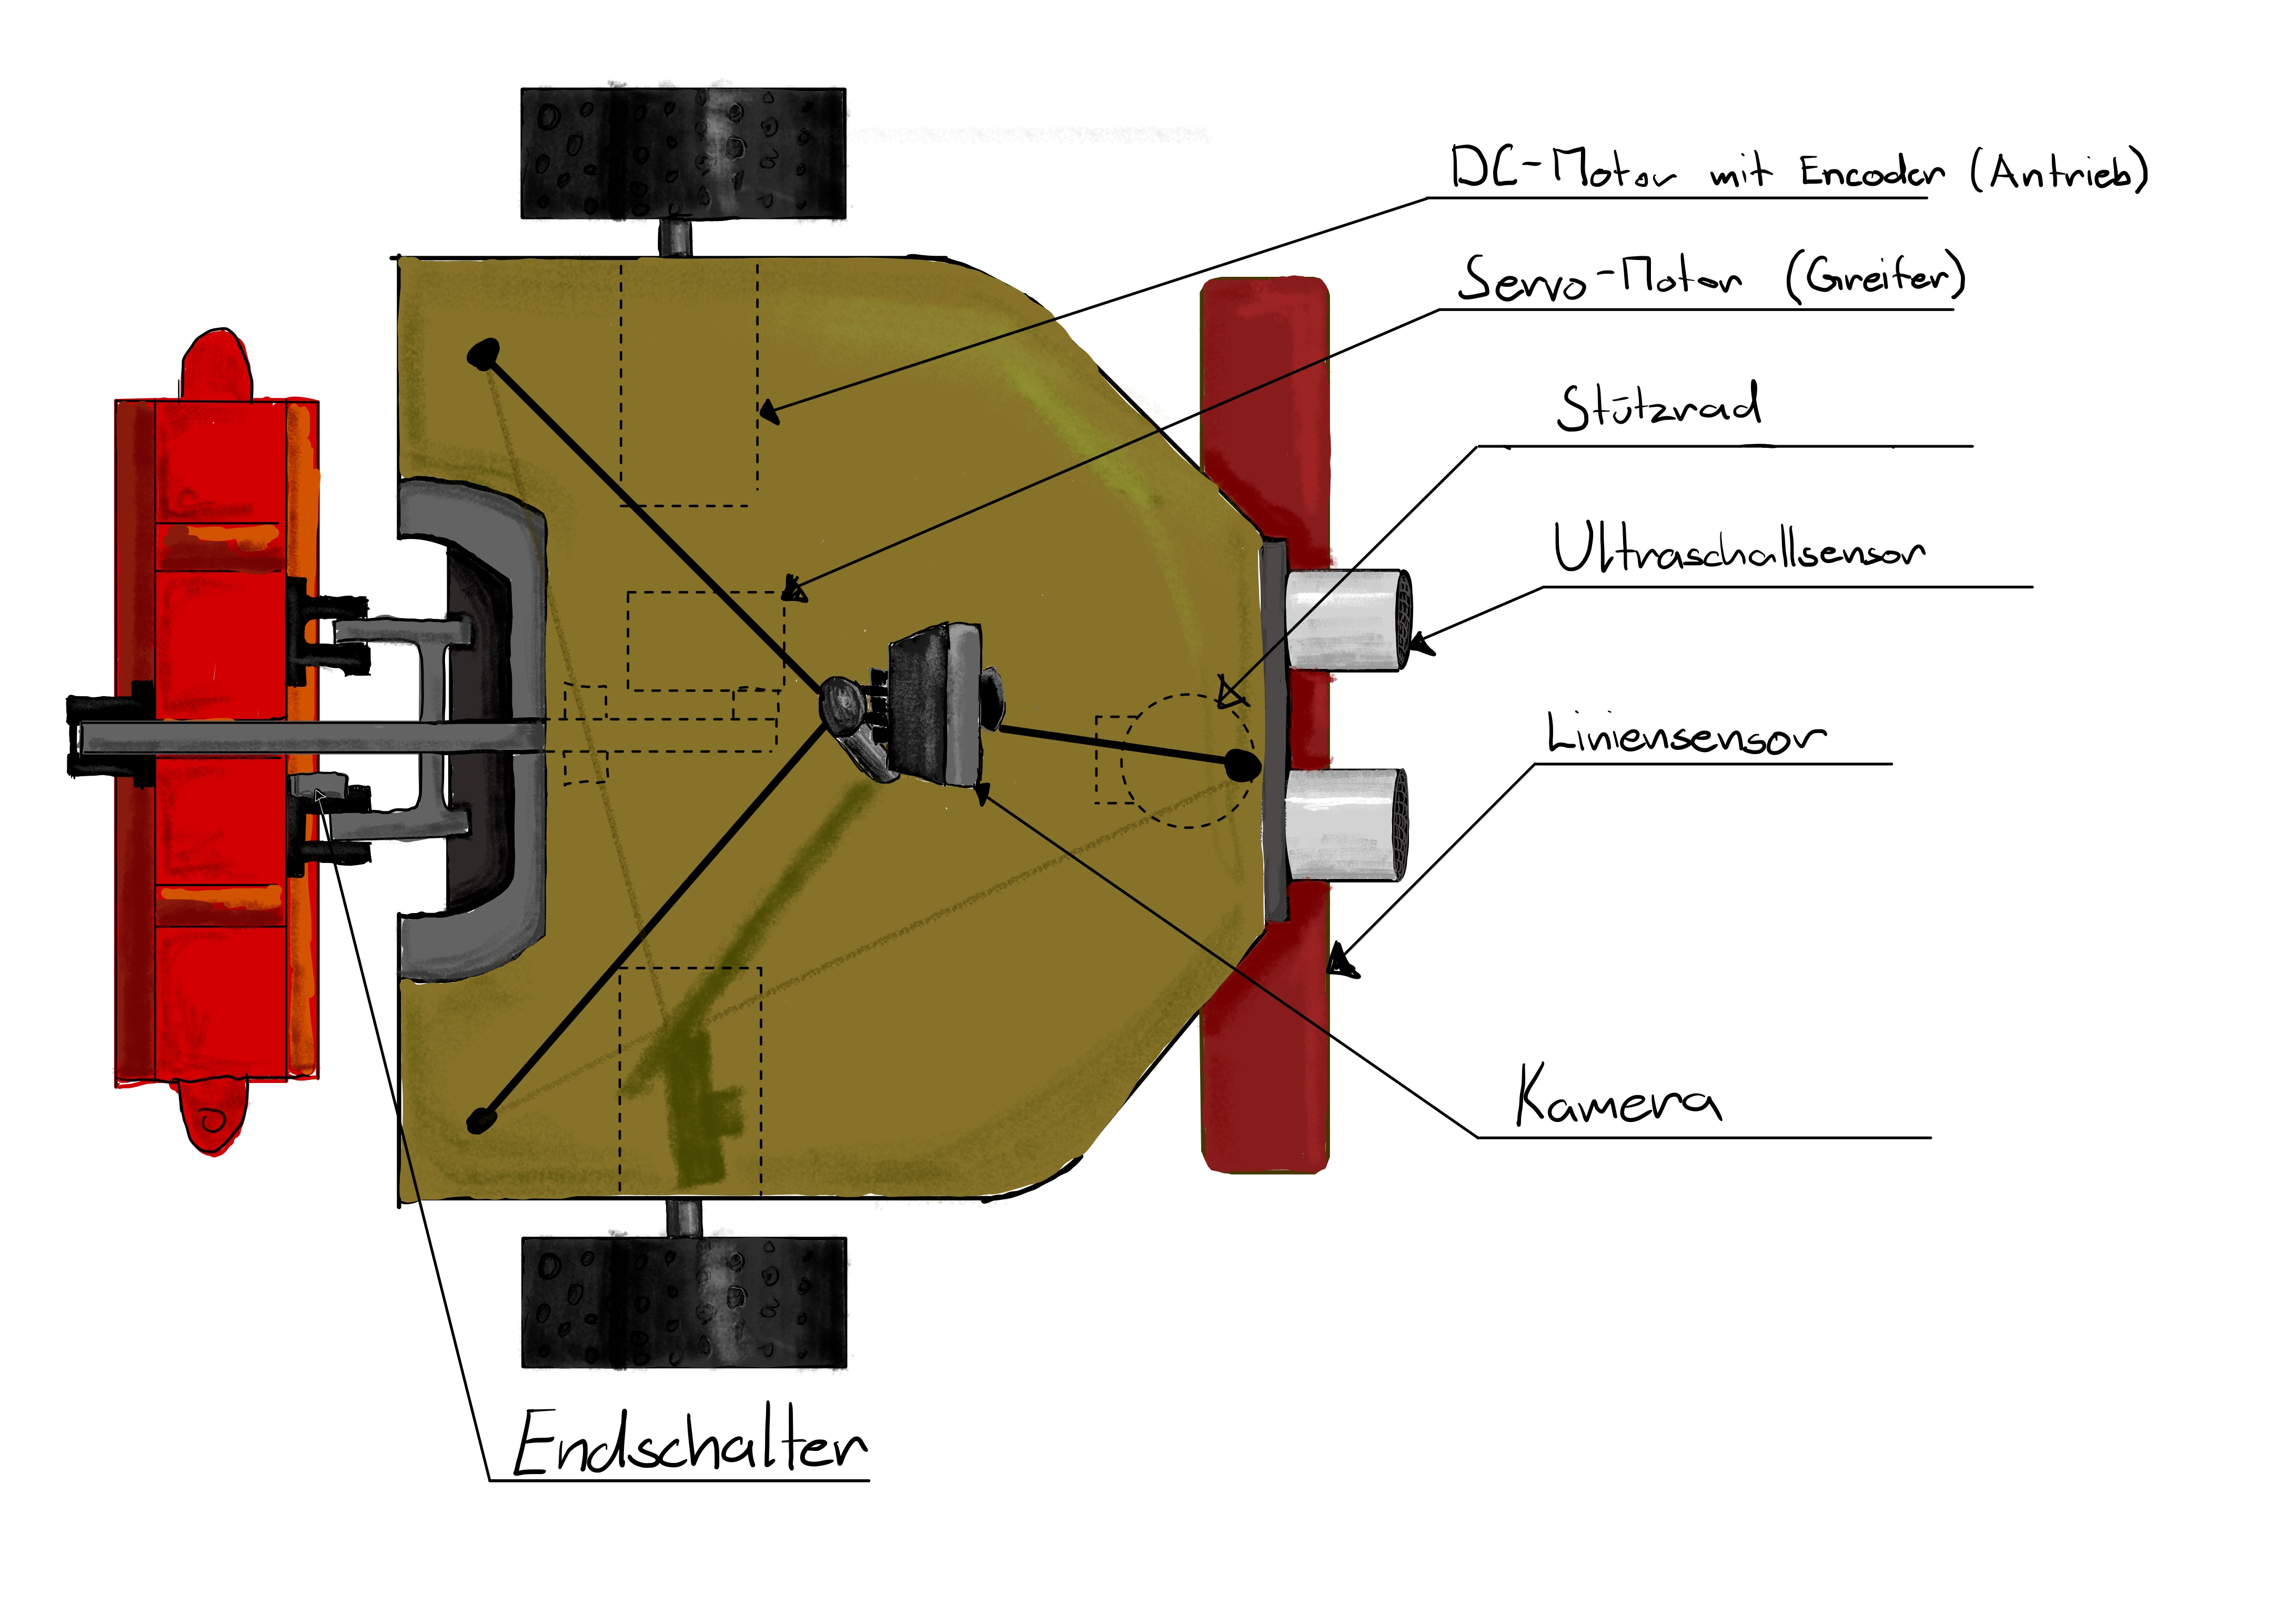
\includegraphics[width=\textwidth]{assets/gesamtkonzept/Skizze-Fahrzeugkonzept-Beschriftet.jpg}
\caption{Konzeptskizze Gesamtkonzept}
\label{fig:robot_concept-scetch_labeld}
\end{figure}

\subsection{Komponenten}
Für das Konzept wurden folgende Komponenten mithilfe der Technologierecherche (siehe Anhang \ref{techrecherche}) und anschliessenden morphologische Kästen (siehe Anhang \ref{mk}) und Nutzwertanalysen (siehe Anhang \ref{nutzwertanalyse}) ermittelt. 

\begin{table}[H]
\centering
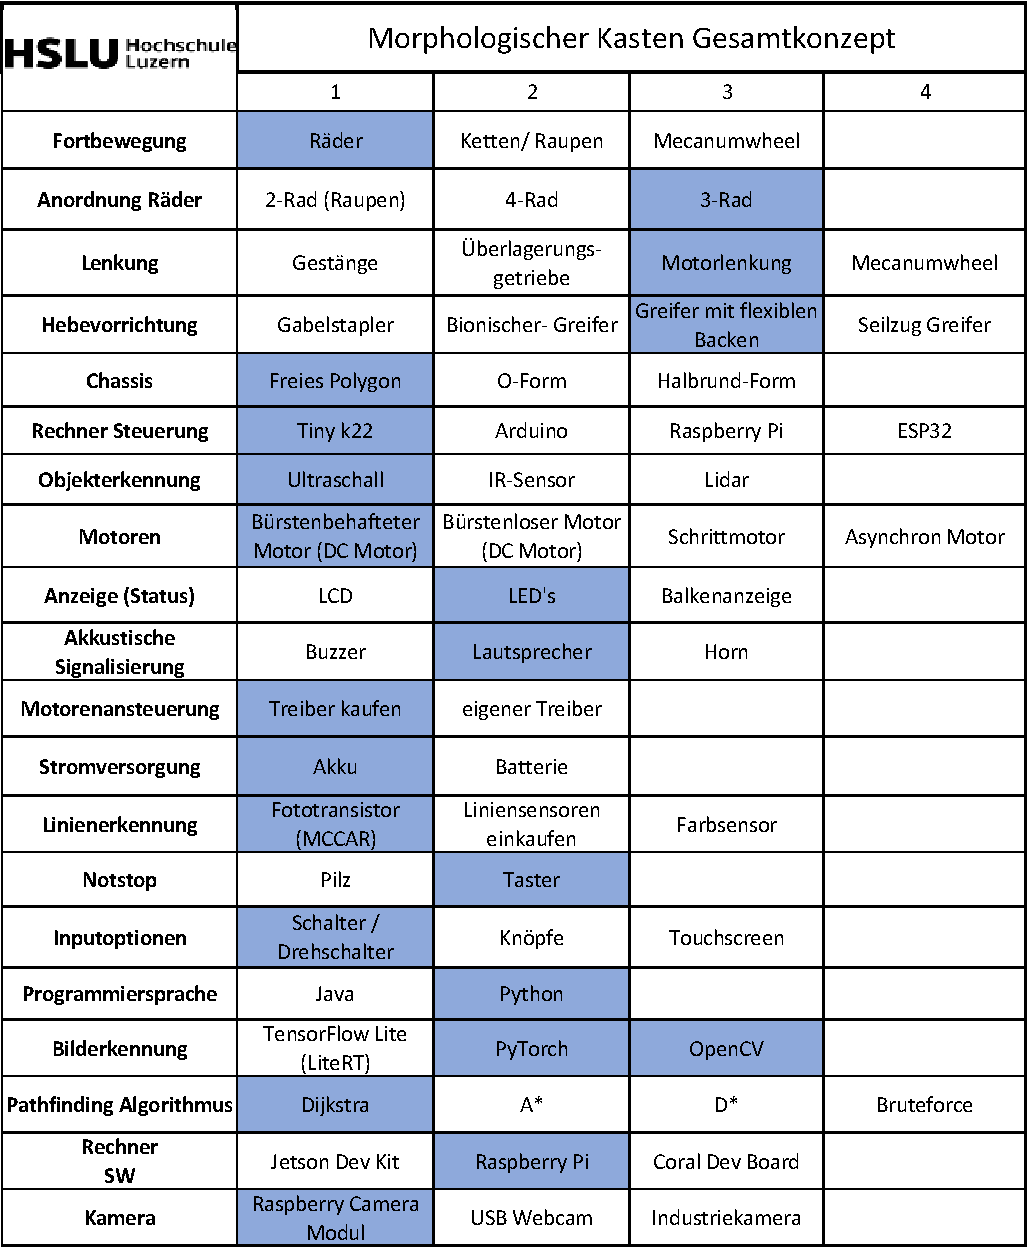
\includegraphics[width=\textwidth -20mm]{assets/MK-all.pdf}
\caption{Morphologischer Kasten: Gesamtkonzept}
\label{table:mk-all}
\end{table}

Es ist geplant einen Roboter in Form eines freien Ploygons zu bauen, der sich mit drei Rädern fortbewegt und eine Motorlenkung besitzt. Hindernisse kann der Roboter dank einem Greifer mit flexiblen Backen anheben. Dies ist in der vorherigen Abbildung \ref{fig:robot_concept-scetch_labeld} ersichtlich .

Die Steuerung wird auf einem \acrshort{tinyk22} betrieben. Die Distanz zu den Objekten wird mittels einem Ultraschallsensor erkannt. Die bürstenbehafteten Motoren werden mit einem gekauften Treiber angesteuert. Die Stromversorgung läuft über einen Akku. Der Akkustand und der Status des Roboters werden durch \acrfull{led} angezeigt. Damit der Roboter die Linien erkennt, wird ein Liniensensor mit Fototransistoren verwendet. Das Ziel wird über einen Drehschalter vom Benutzer ausgewählt.
Wenn der Roboter das Ziel erreicht, verkündet er dies über einen Lautsprecher. Im Notfall wird der Roboter über einen Taster ausgeschaltet.

Die Bildverarbeitung und Navigation werden in Python programmiert und laufen auf einem Raspberry Pi. Zur Bilderkennung wird eine Kombination von PyTorch und OpenCV verwendet. Die Bilder werden mit einer Raspberry Pi Camera aufgenommen. Der kürzeste Weg wird mit einem Dijkstra Algorithmus berechnet.

\subsection{Ablauf}

Der Ablauf einer Durchfahrt ist im Ablaufdiagramm \ref{fig:ablaufdiagramm} aufgezeigt.
Die Schritte, die mit einem Plus markiert sind, sind in den folgenden Kapiteln als Subprozesse detailliert definiert.

\begin{figure}[H]
\centering
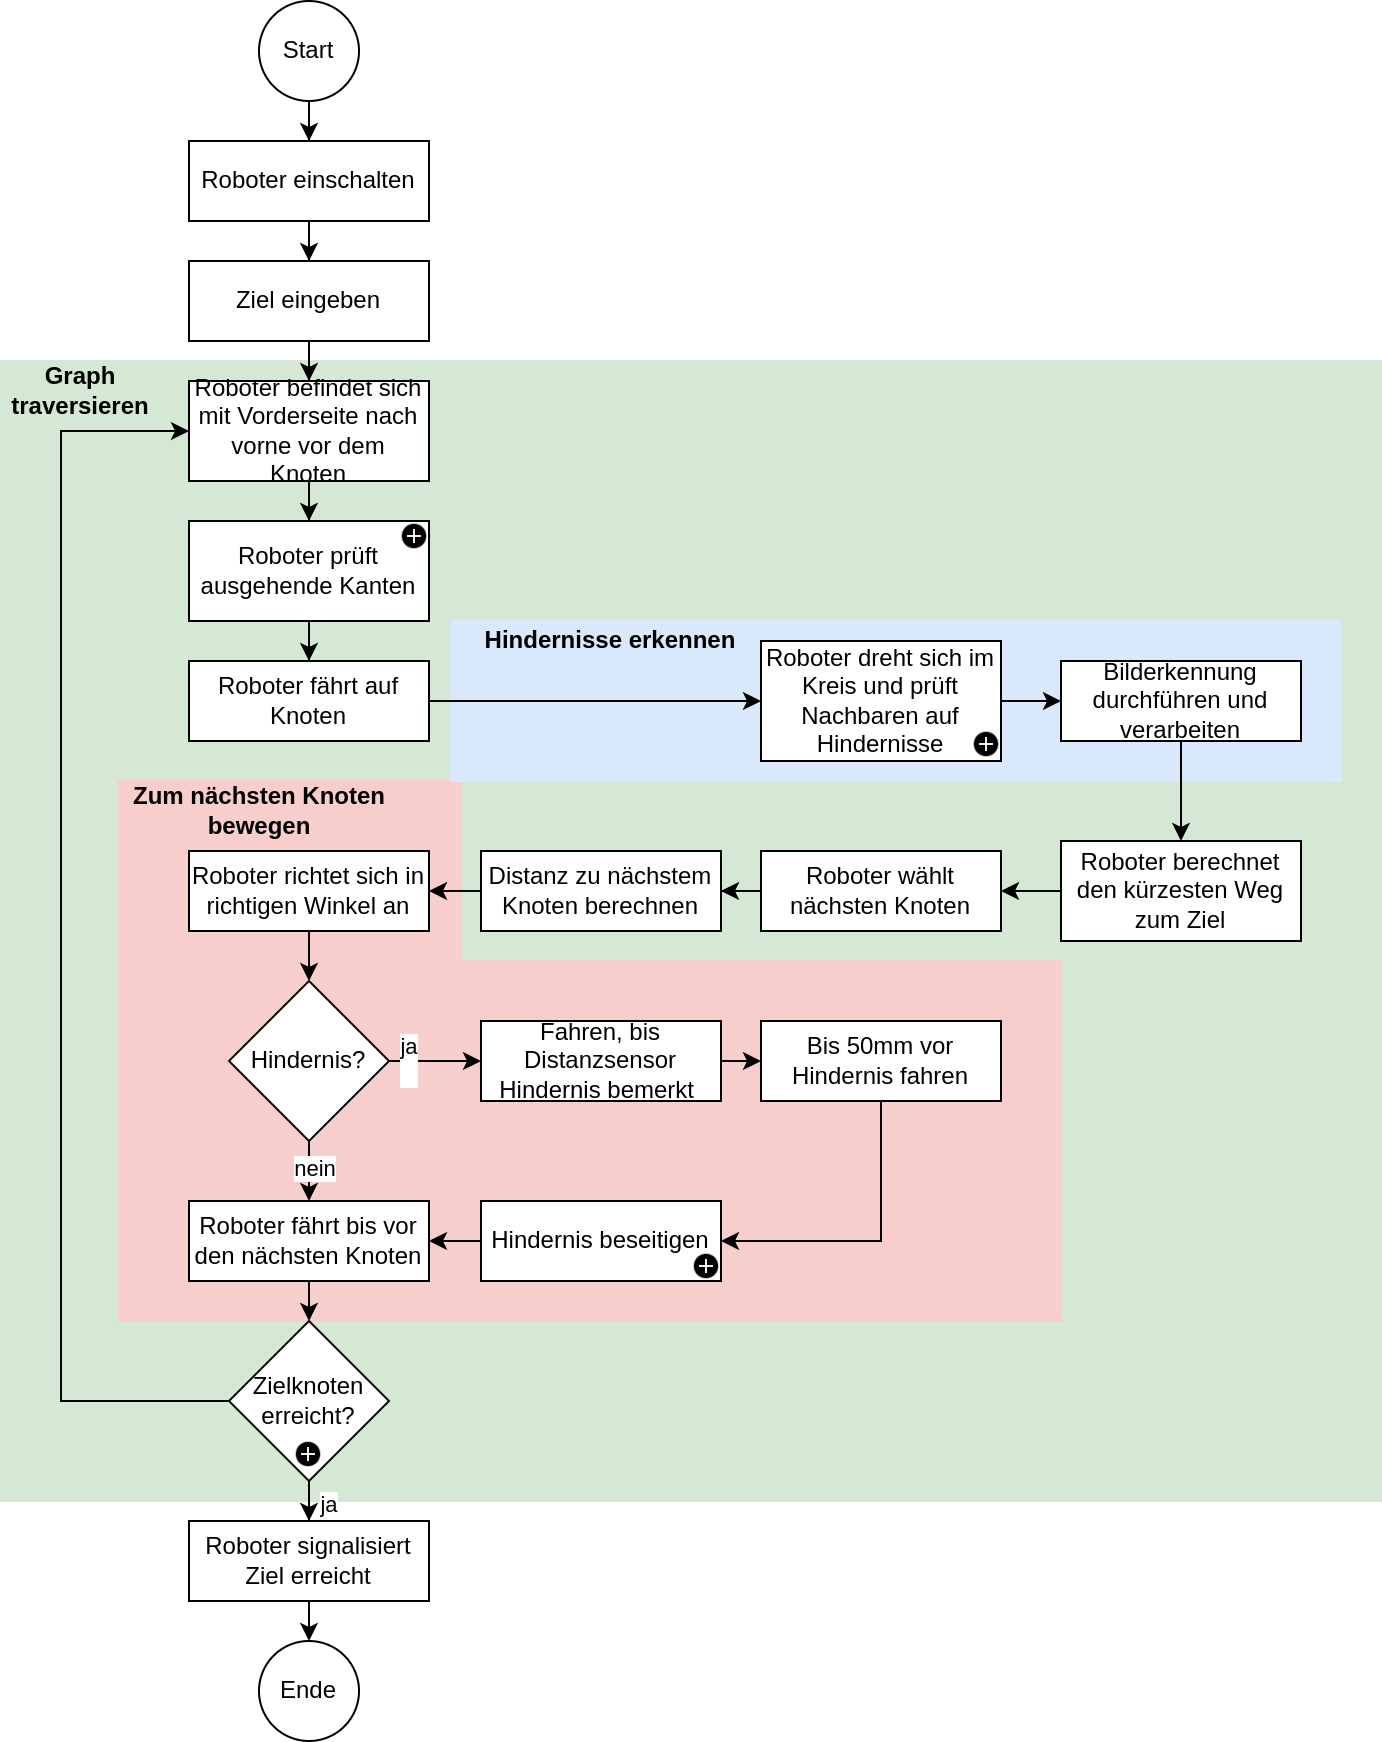
\includegraphics[width=\textwidth]{assets/gesamtkonzept/ablaufdiagramm.png}
\caption{Ablaufdiagramm}
\label{fig:ablaufdiagramm}
\end{figure}

\subsubsection{Ausgehende Kanten erkennen}

Um alle ausgehenden Kanten und deren Winkel zu erkennen, wird der folgende Ablauf in Abbildung \ref{fig:ablaufdiagramm} durchlaufen. Dies ist nötig, damit der Roboter weiss, in welche Richtung er sich drehen muss, um auf die nächste Kante zu gelangen. Ebenfalls können so fehlende Linien erkannt werden.

\begin{figure}[H]
\centering
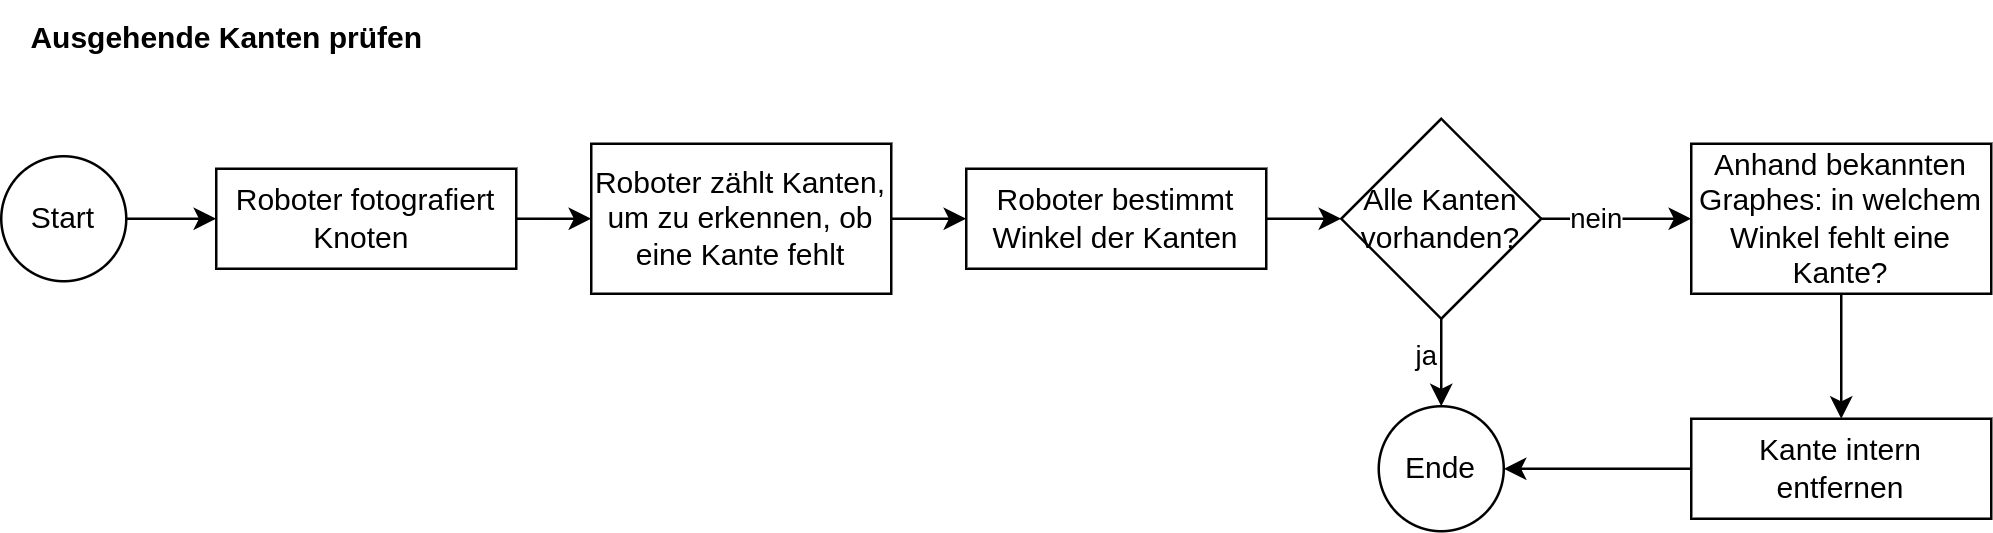
\includegraphics[width=\textwidth]{assets/gesamtkonzept/ablaufdiagramm-kanten-erkennen.png}
\caption{Ablaufdiagramm ausgehende Kanten erkennen}
\label{fig:ablaufdiagramm-kanten-erkennen}
\end{figure}

Der Roboter bewegt sich auf einen Knoten zu und hält 15 cm vor diesem an. Der Knoten wird fotografiert und der Roboter fährt anschliessend auf den Knoten. Das Bild wird rotiertet und mit OpenCV zuerst so entzerrt, sodass der Knoten gerade von oben dargestellt wird. Danach werden die einzelnen Winkel gemessen. Dies ist im Prototyping Kapitel im Anhang \ref{winkelerkennung} ausführlicher beschrieben. Das Resultat dieser Objekterkennung ist eine Liste mit Winkeln.

\begin{figure}[H]
\centering
\begin{subfigure}{0.45\textwidth}
\centering
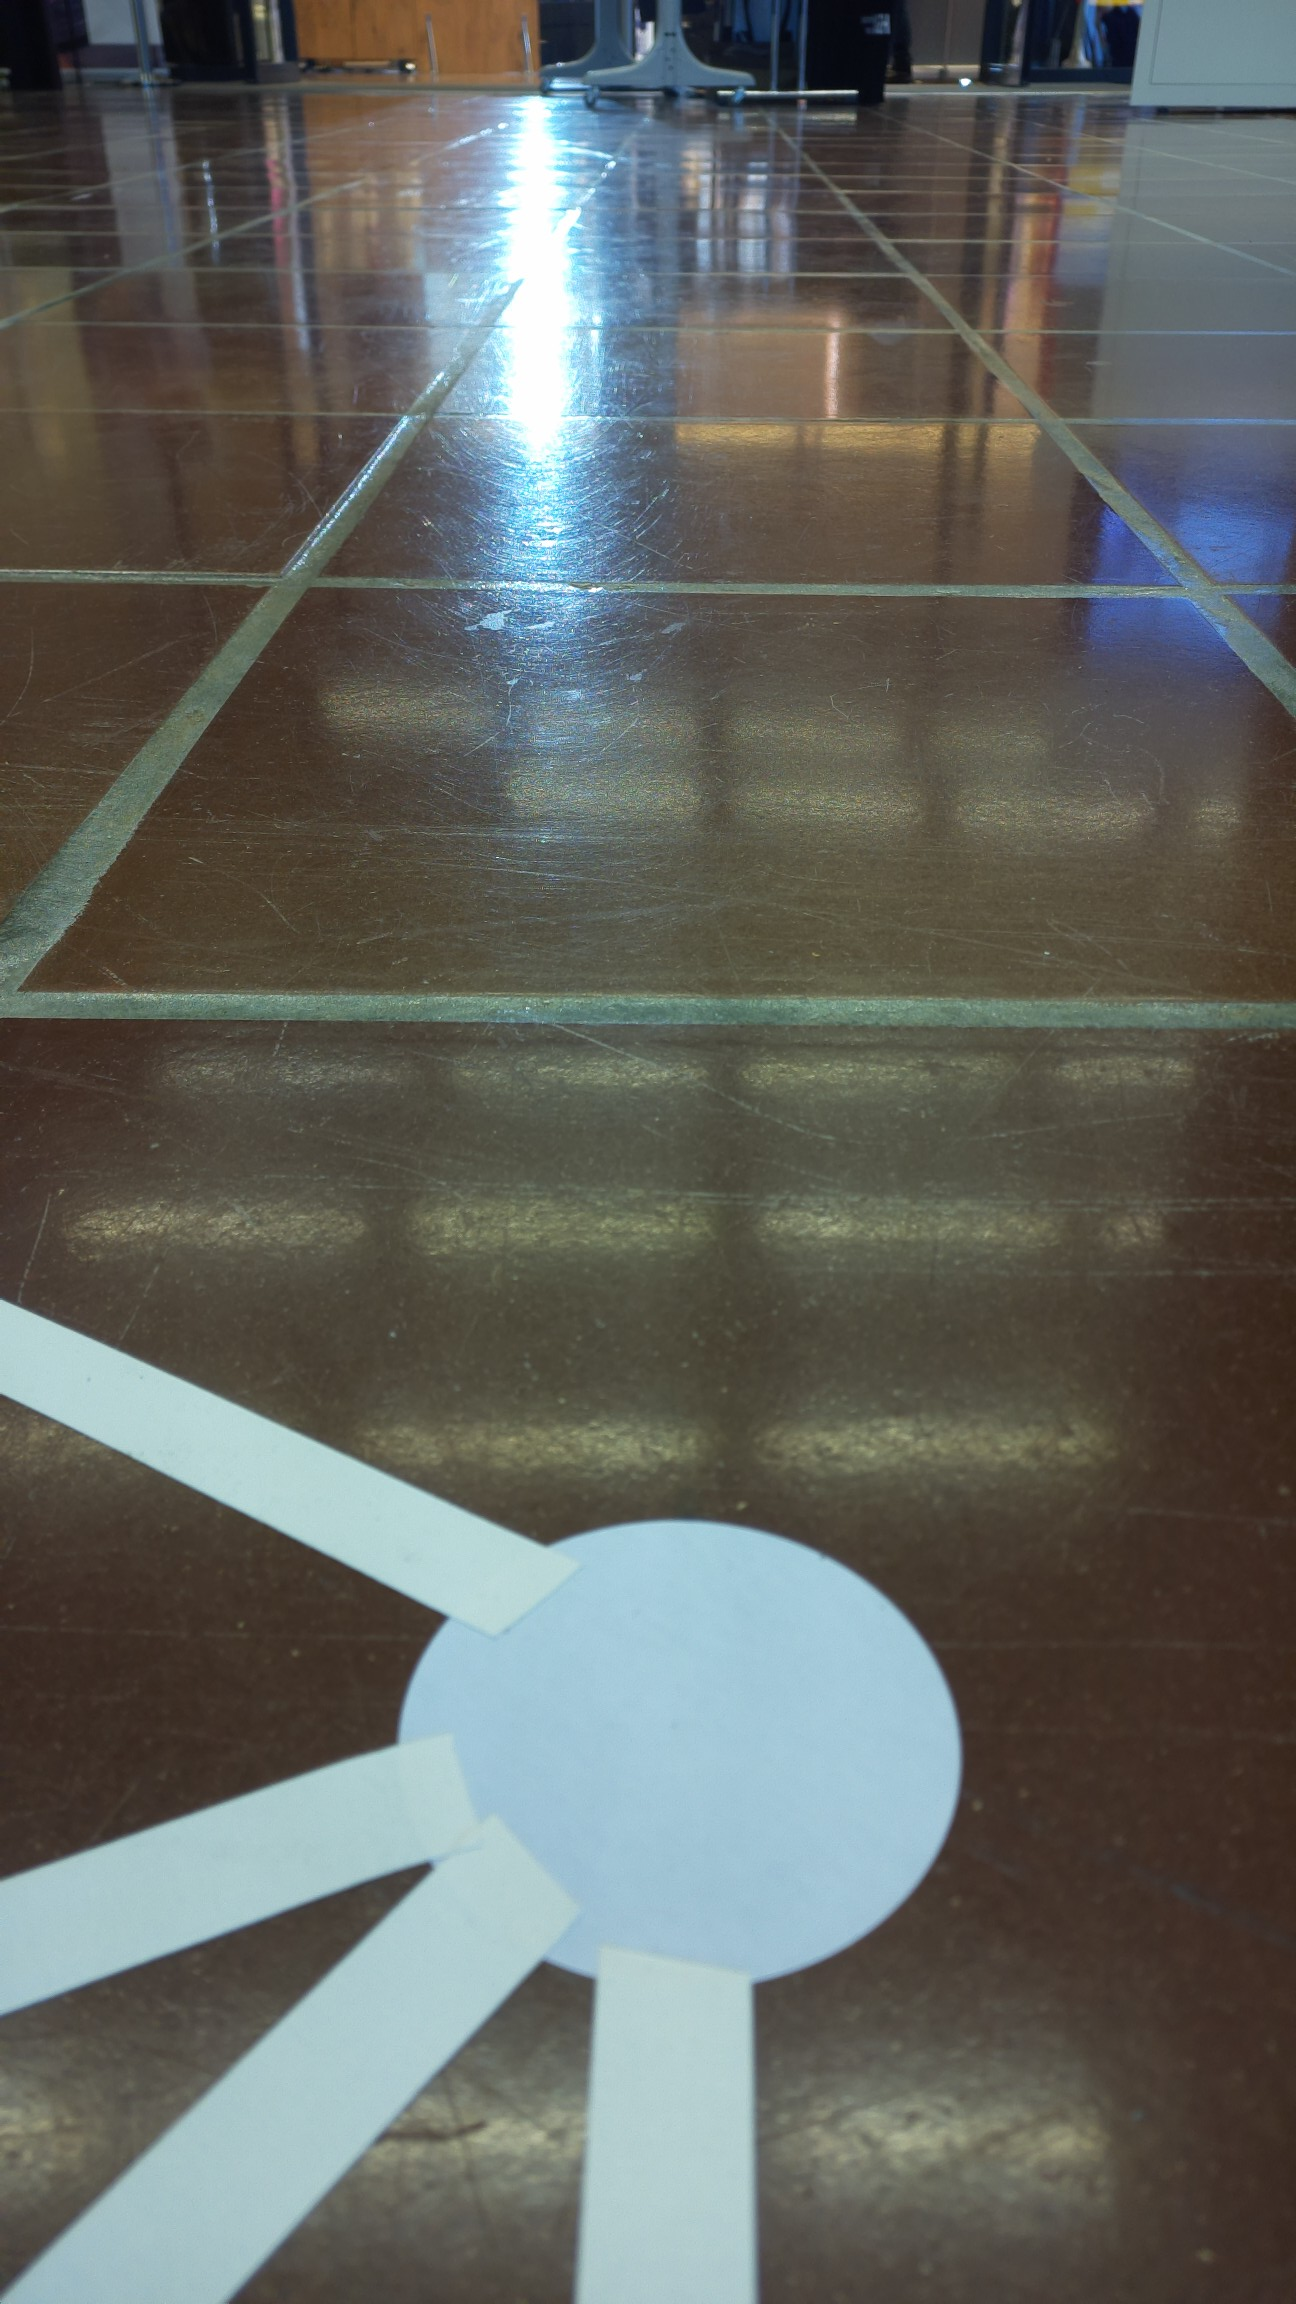
\includegraphics[width=0.95\linewidth]{assets/informatik-prototyp/opencv/angle_detection/image_taken_by_pi_camer_before_node.jpg} 
\caption{Knoten mit 15cm Abstand}
\label{fig:node-15cm-before}
\end{subfigure}
\begin{subfigure}{0.45\textwidth}
\centering
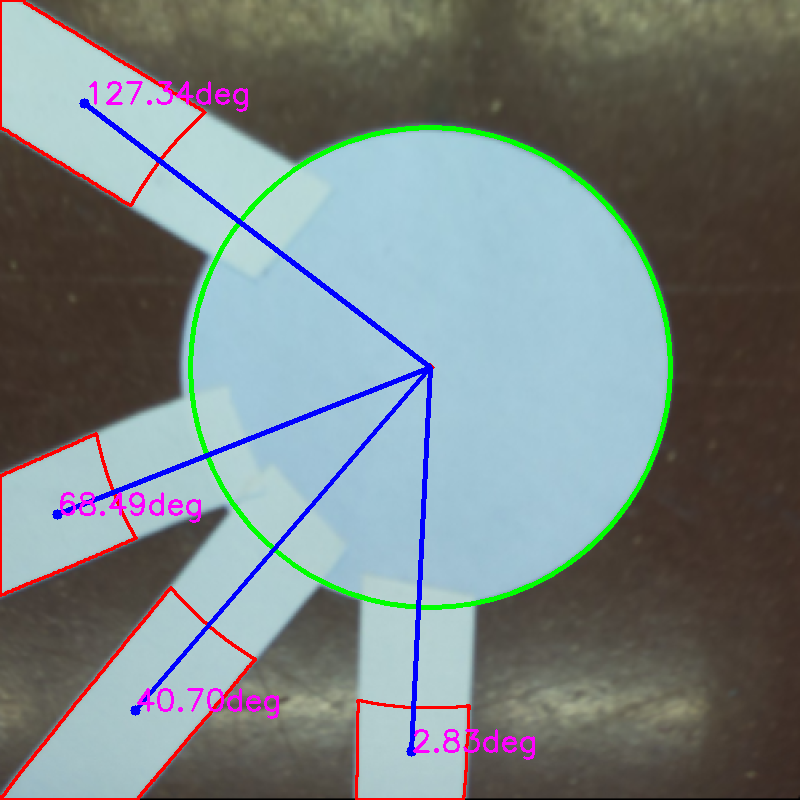
\includegraphics[width=0.95\linewidth]{assets/informatik-prototyp/opencv/angle_detection/node_with_edge_angles_annotated.png} 
\caption{Knoten mit gemessenen Winkeln}
\label{fig:node-angles}
\end{subfigure}

\caption{Winkelerkennung}
\label{fig:angle-recognition}
\end{figure}

Die erhaltene Liste mit Winkeln wird nun verwendet, um mögliche fehlende Linien zu erkennen und die Winkel intern zu speichern. Die internen Winkel werden verwendet, um den Roboter richtig auszurichten, wenn dieser auf die nächste Linie fährt.

Der Roboter selber hat einen Grundgraphen mit Winkeln gespeichert. Diese Winkel ergeben sich aus dem zur Verfügung gestellten Graph.
Da der Graph nicht genau so aufgeklebt sein wird, wie auf der Skizze, wurden Bereiche definiert, in denen sich die Winkel befinden sollten.

Ein Ausschnitt, der zeigt, wie der interne Graph in einem YAML File definiert ist, ist hier eingefügt.

\begin{verbatim}
C: [{D: [60, [30, 120]}, {B: [240, [120, 30]}, {H: [60, [30, 30]}]
\end{verbatim}

Auf Grafik a) sind alle Winkel eingezeichnet inklusive der Halbwinkel zwischen allen Kanten. In Grafik b) ist die Kante zwischen C und D gezeigt, dies entspricht \verb|'C: [{D: [60, [30, 120]}'| im YAML File. 
Wenn der Roboter sich von Knoten C zu Knoten D bewegen möchte, dann wäre diese Kante im Idealfall 60\textdegree\ von der Kante links aus. Das der Idealfall nicht eintreten wird, sind die Halbwinkel eingezeichnet, hier 30\textdegree\ und 120\textdegree. Von der linksliegenden Kante aus, darf kann sich die Kante zu Knoten D also im Bereich von 60\textdegree-30\textdegree\ und 60\textdegree+120\textdegree, sprich 30\textdegree\ und 180\textdegree\ befinden. Befindet sich eine gemessene Kante in diesem Bereich, wird es die Kante C zu D sein.

\begin{figure}[H]
\centering
\begin{subfigure}{0.65\textwidth}
\centering
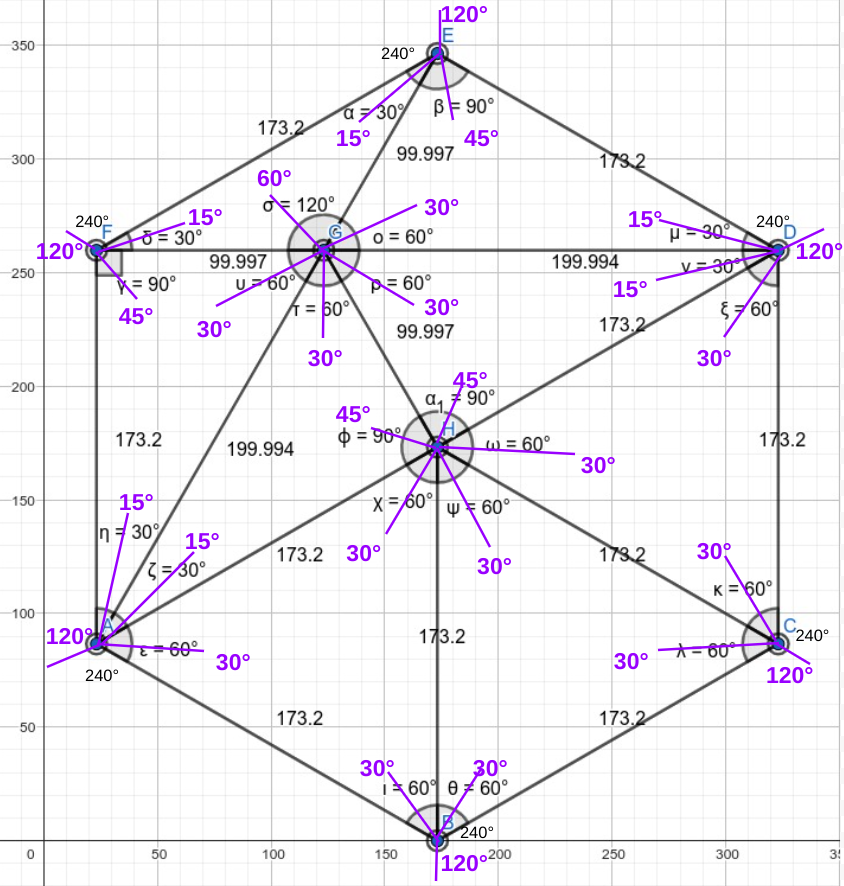
\includegraphics[width=0.95\linewidth]{assets/informatik-prototyp/graph-angles.png} 
\caption{Graph mit Winkeln und Winkelbereichen}
\label{fig:angled-graph}
\end{subfigure}
\begin{subfigure}{0.32\textwidth}
\centering
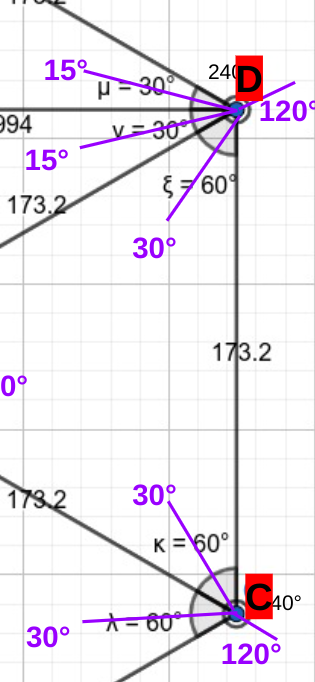
\includegraphics[width=0.95\linewidth]{assets/informatik-prototyp/c-d-angle-labeled.png} 
\caption{C zu D Winkel}
\label{fig:excerpt-angled-graph}
\end{subfigure}
\caption{Winkel im Graphen}
\label{fig:angles}
\end{figure}

Als erstes wird die Länge der Liste mit Winkeln gemessen. Wenn sich gleich viele Winkel darin befinden, wie es laut dem Grundgraphen ausgehende Linie haben soll, dann bedeutet das, dass keine Linie fehlt. In diesem Fall werden die internen Winkel mit den tatsächlichen Werten aktualisiert.

Falls es weniger Winkel gibt als erwartet, werden die erhaltenen Winkel zu den einzelnen möglichen Bereichen zugeordnet. In dem Bereich, in welchem kein Winkel zugeordnet wurde, fehlt eine Linie. Folglich aktualisiert der Roboter seine internen Informationen: eine Linie wird aus dem Grundgraphen entfernt und die anderen Winkel werden mit den gemessenen Werten ersetzt.

Nachdem der Roboter den nächsten Knoten berechnet hat, wird der Winkel zur richtigen ausgehenden Kante an die Steuerung gesendet. Der Roboter dreht sich, um auf dieser Linie weiterzufahren.

\subsubsection{Zielknoten erkennen}

Damit der Roboter überprüfen kann, ob er wirklich das Ziel erreicht hat, muss erkannt werden können, ob der Knoten der richtige Zielknoten ist. Dazu wird der \acrfull{orb} Algorithmus verwendet, der Teil der OpenCV Bibliothek ist.\gls{orb-gloss} lernt die Merkmale von Objekten und erkennt auf einem Bild, welches Objekt gefunden wurde.

Der Algorithmus wird so eingesetzt werden, dass der Roboter bevor er den Lauf beginnt die Merkmal der drei Buchstaben lernt. Jedes Mal, wenn ein Knoten fotografiert wird, um die ausgehenden Kanten zu prüfen, wird ebenfalls geprüft, ob sich ein Buchstaben darauf befindet. Falls ein Buchstaben detektiert wird, bestimmt \acrshort{orb} um welchen es sich handelt.

Dadurch dass \acrshort{orb} die Merkmale der Buchstaben detektiert, ist es nicht nötig, die Rotation der Buchstaben zu beachten. Unabhängig von welcher Richtung der Roboter den Zielknoten fotografiert, kann der Buchstabe erkannt werden.

Auf der folgenden Grafik \ref{fig:orb-zielknoten-konzept} wird mit den farbigen Linien dargestellt, wie \acrshort{orb} die bekannten Merkmale (jeweils linkes Bild) in den zu analysierenden Bildern (jeweils rechtes Bild) findet.

\begin{figure}[H]
\centering
\begin{subfigure}{0.3\textwidth}
\centering
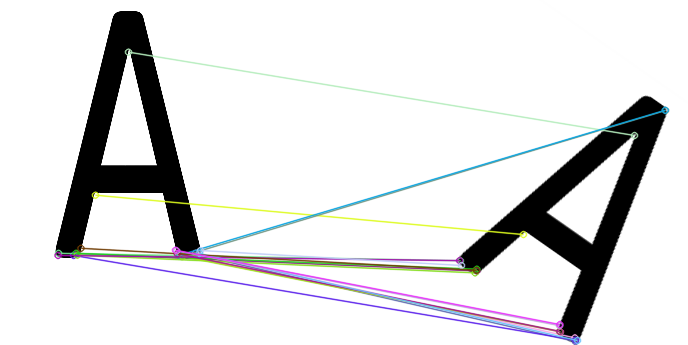
\includegraphics[width=0.95\linewidth]{assets/informatik-prototyp/opencv/target_node_detection/orb-a.png} 
\caption{ORB A}
\label{fig:orb-a-konzept}
\end{subfigure}
\begin{subfigure}{0.3\textwidth}
\centering
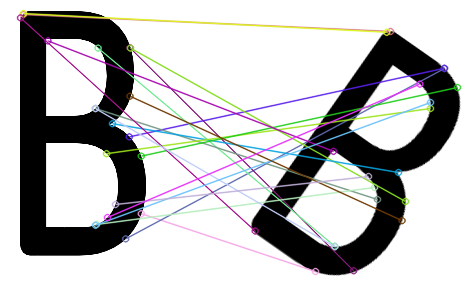
\includegraphics[width=0.95\linewidth]{assets/informatik-prototyp/opencv/target_node_detection/orb-b.png} 
\caption{ORB B}
\label{fig:orb-b-konzept}
\end{subfigure}
\begin{subfigure}{0.3\textwidth}
\centering
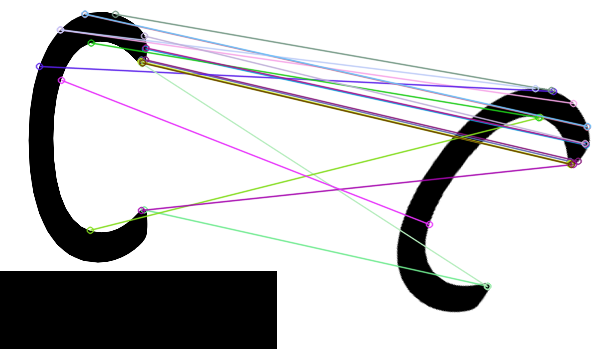
\includegraphics[width=0.95\linewidth]{assets/informatik-prototyp/opencv/target_node_detection/orb-c.png} 
\caption{ORB C}
\label{fig:orb-c-konzept}
\end{subfigure}

\caption{Zielknotenerkennung mit ORB}
\label{fig:orb-zielknoten-konzept}
\end{figure}


Mit \acrshort{orb} werden nur die Buchstaben A, B oder C erkannt, da der trainierte Algorithmus nur diese drei Zeichen kennt. So kann ausgeschlossen werden, dass ein C beispielsweise als das Klammer Zeichen \verb|(| erkannt werden würde.


\subsubsection{Pylonen und Hindernisse erkennen}

Damit der Roboter weiss, ob sich eine Pylone auf einem Nachbarsknoten oder eine Barriere auf einer ausgehenden Linie befindet, wird der Ablauf auf Abbildung \ref{fig:image-detection-obstacles} durchgeführt.

\begin{figure}[H]
\centering
\begin{subfigure}{0.45\textwidth}
\centering
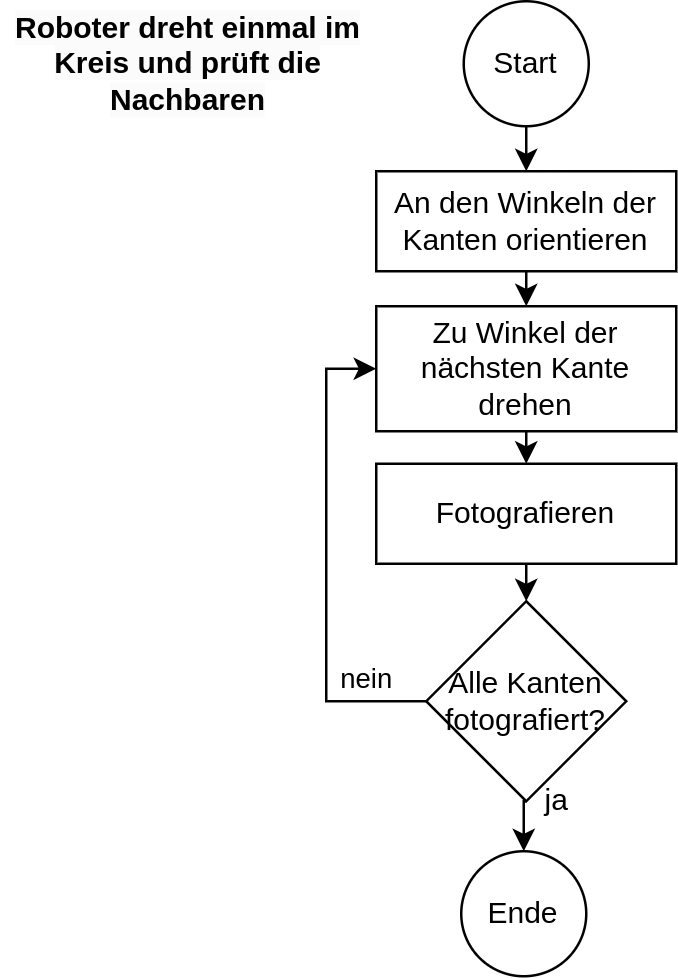
\includegraphics[width=0.95\textwidth]{assets/gesamtkonzept/ablaufdiagramm-hindernisse-erkennen.png}
\caption{Ablaufdiagramm Hindernis erkennen}
\label{fig:ablaufdiagramm-hindernis-erkennen}
\end{subfigure}
\begin{subfigure}{0.5\textwidth}
\centering
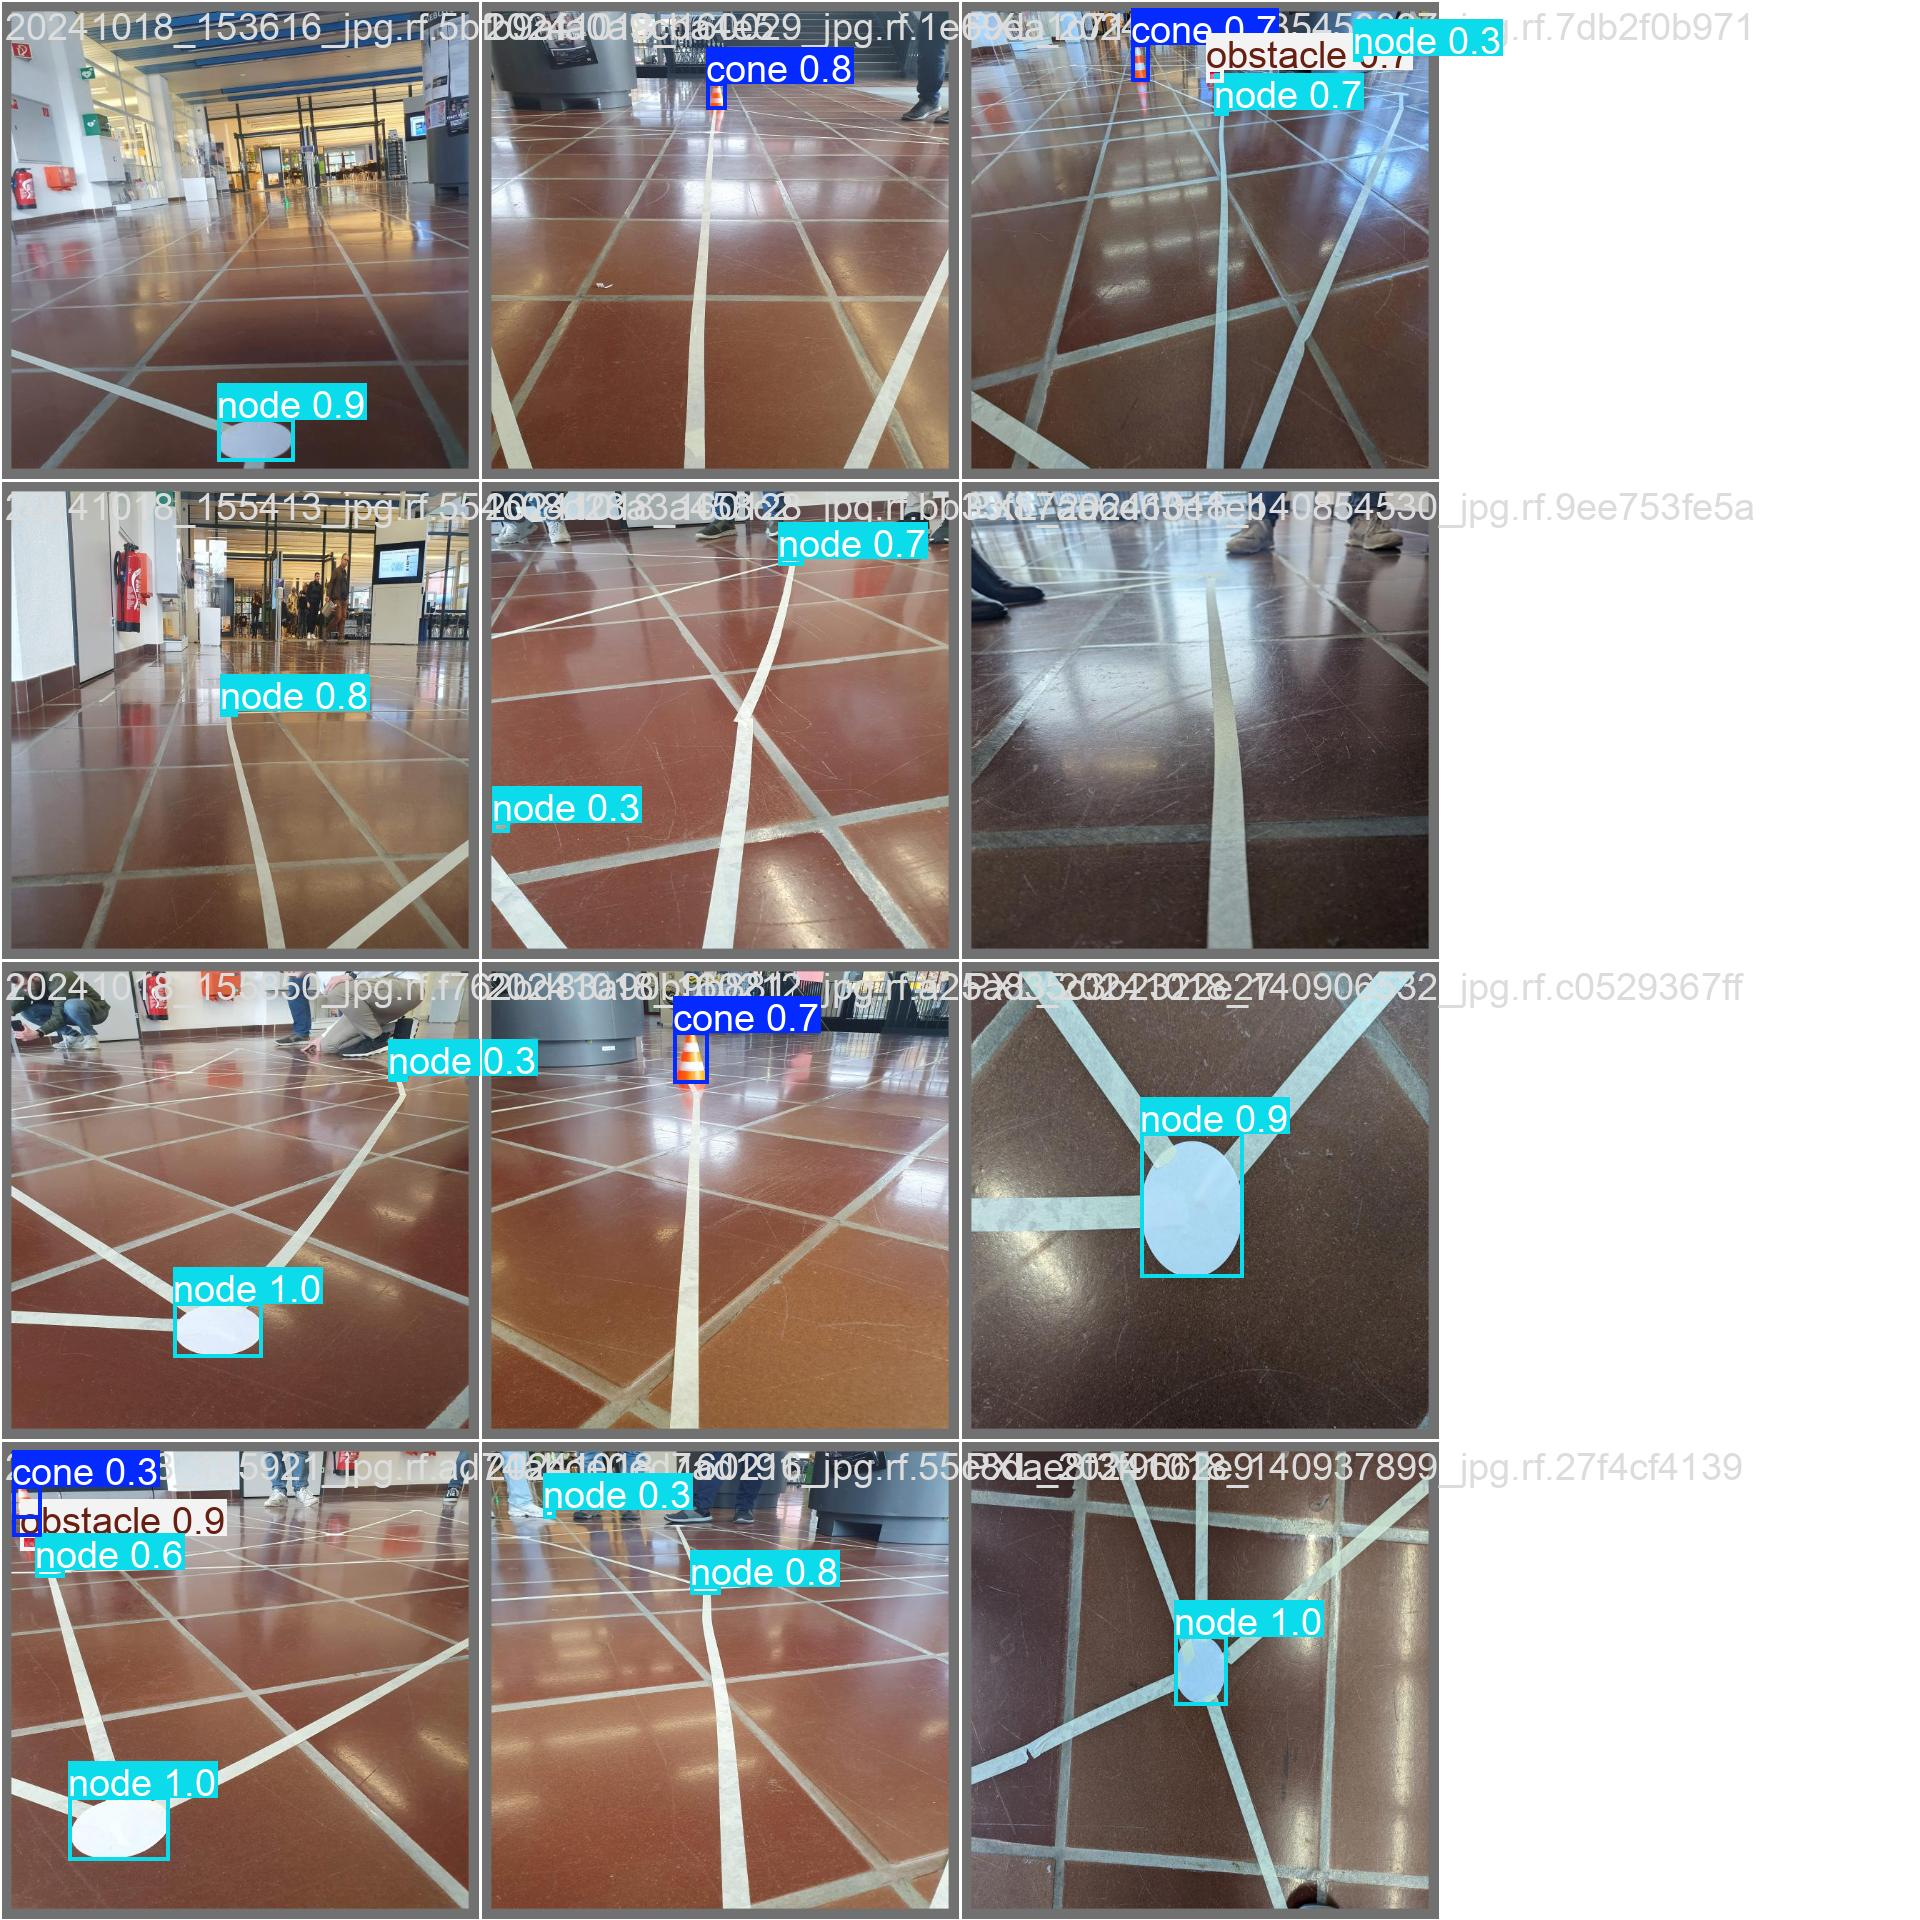
\includegraphics[width=0.95\textwidth]{assets/informatik-prototyp/yolo/recognized-images.jpeg}
\caption{YOLOv11 Bilderkennung}
\label{fig:img-recognition-yolo-concept}
\end{subfigure}
\caption{Bilderkennung Hindernisse}
\label{fig:image-detection-obstacles}
\end{figure}

Aus dem vorherigen Schritt der Kanten erkennen, kennt der Roboter alle ausgehenden Linien und deren Position. Er dreht sich nun im Uhrzeigersinn zu jeder Kante und fotografiert diese. Durch das Hochformat der Kameras sieht er weit und kann auch nur die wichtigen Elemente sehen, sprich, diese, die sich auf der Linie befinden.

Die Bilder werden mit einem YOLO Objekterkennungsalgorithmus ausgewertet. Dabei werden sowohl Knoten, als auch Pylonen und Barrieren erkannt. Das erhaltene Resultat beschreibt anhand der definierten Klassen welche Elemente erkannt wurden und mithilfe der Koordinaten wo sich diese auf dem Bild befinden.
Alle Hindernisse werden intern gespeichert indem die jeweiligen Kanten höher gewichtet werden.


\newpage

\subsubsection{Hindernisse bewegen}
\label{subsubsection:Hindernisse bewegen}

Um ein vorhandenes Hindernis zu bewegen wird ein Mechanismus zum Anheben, nachfolgend Greifer genannt, verwendet. Nach dem Anheben bewegt sich der Roboter und setzt das Hindernis an der alten Position ab.
Mit nur einem Motor wird das Hindernis eingeklemmt, zentriert und angehoben. Dieser Vorgang und der Aufbau des Greifers wird in folgendem Kapitel erläutert.

Die gezeigten Abbildungen des Greifers stammen von einem Prototyp und stellen nicht das finale Design dar. Sie dienen lediglich zur Veranschaulichung der Funktionsweise. Die Dimensionen des Gestänges sowie die Positionen der Lagerstellen sollen für die finale Variante beibehalten werden.

In der Nutzwertanalyse (Anhang \ref{nutzwertanalyse}) hat man sich zum Anheben des Hindernisses für ein Klemm-Design entschieden, welcher das Hindernis oben an der längsten Kante an 3 Punkten einspannt (siehe Abb. \ref{fig:obstacle_clamping_concept}). 


\begin{figure}[H]
\centering
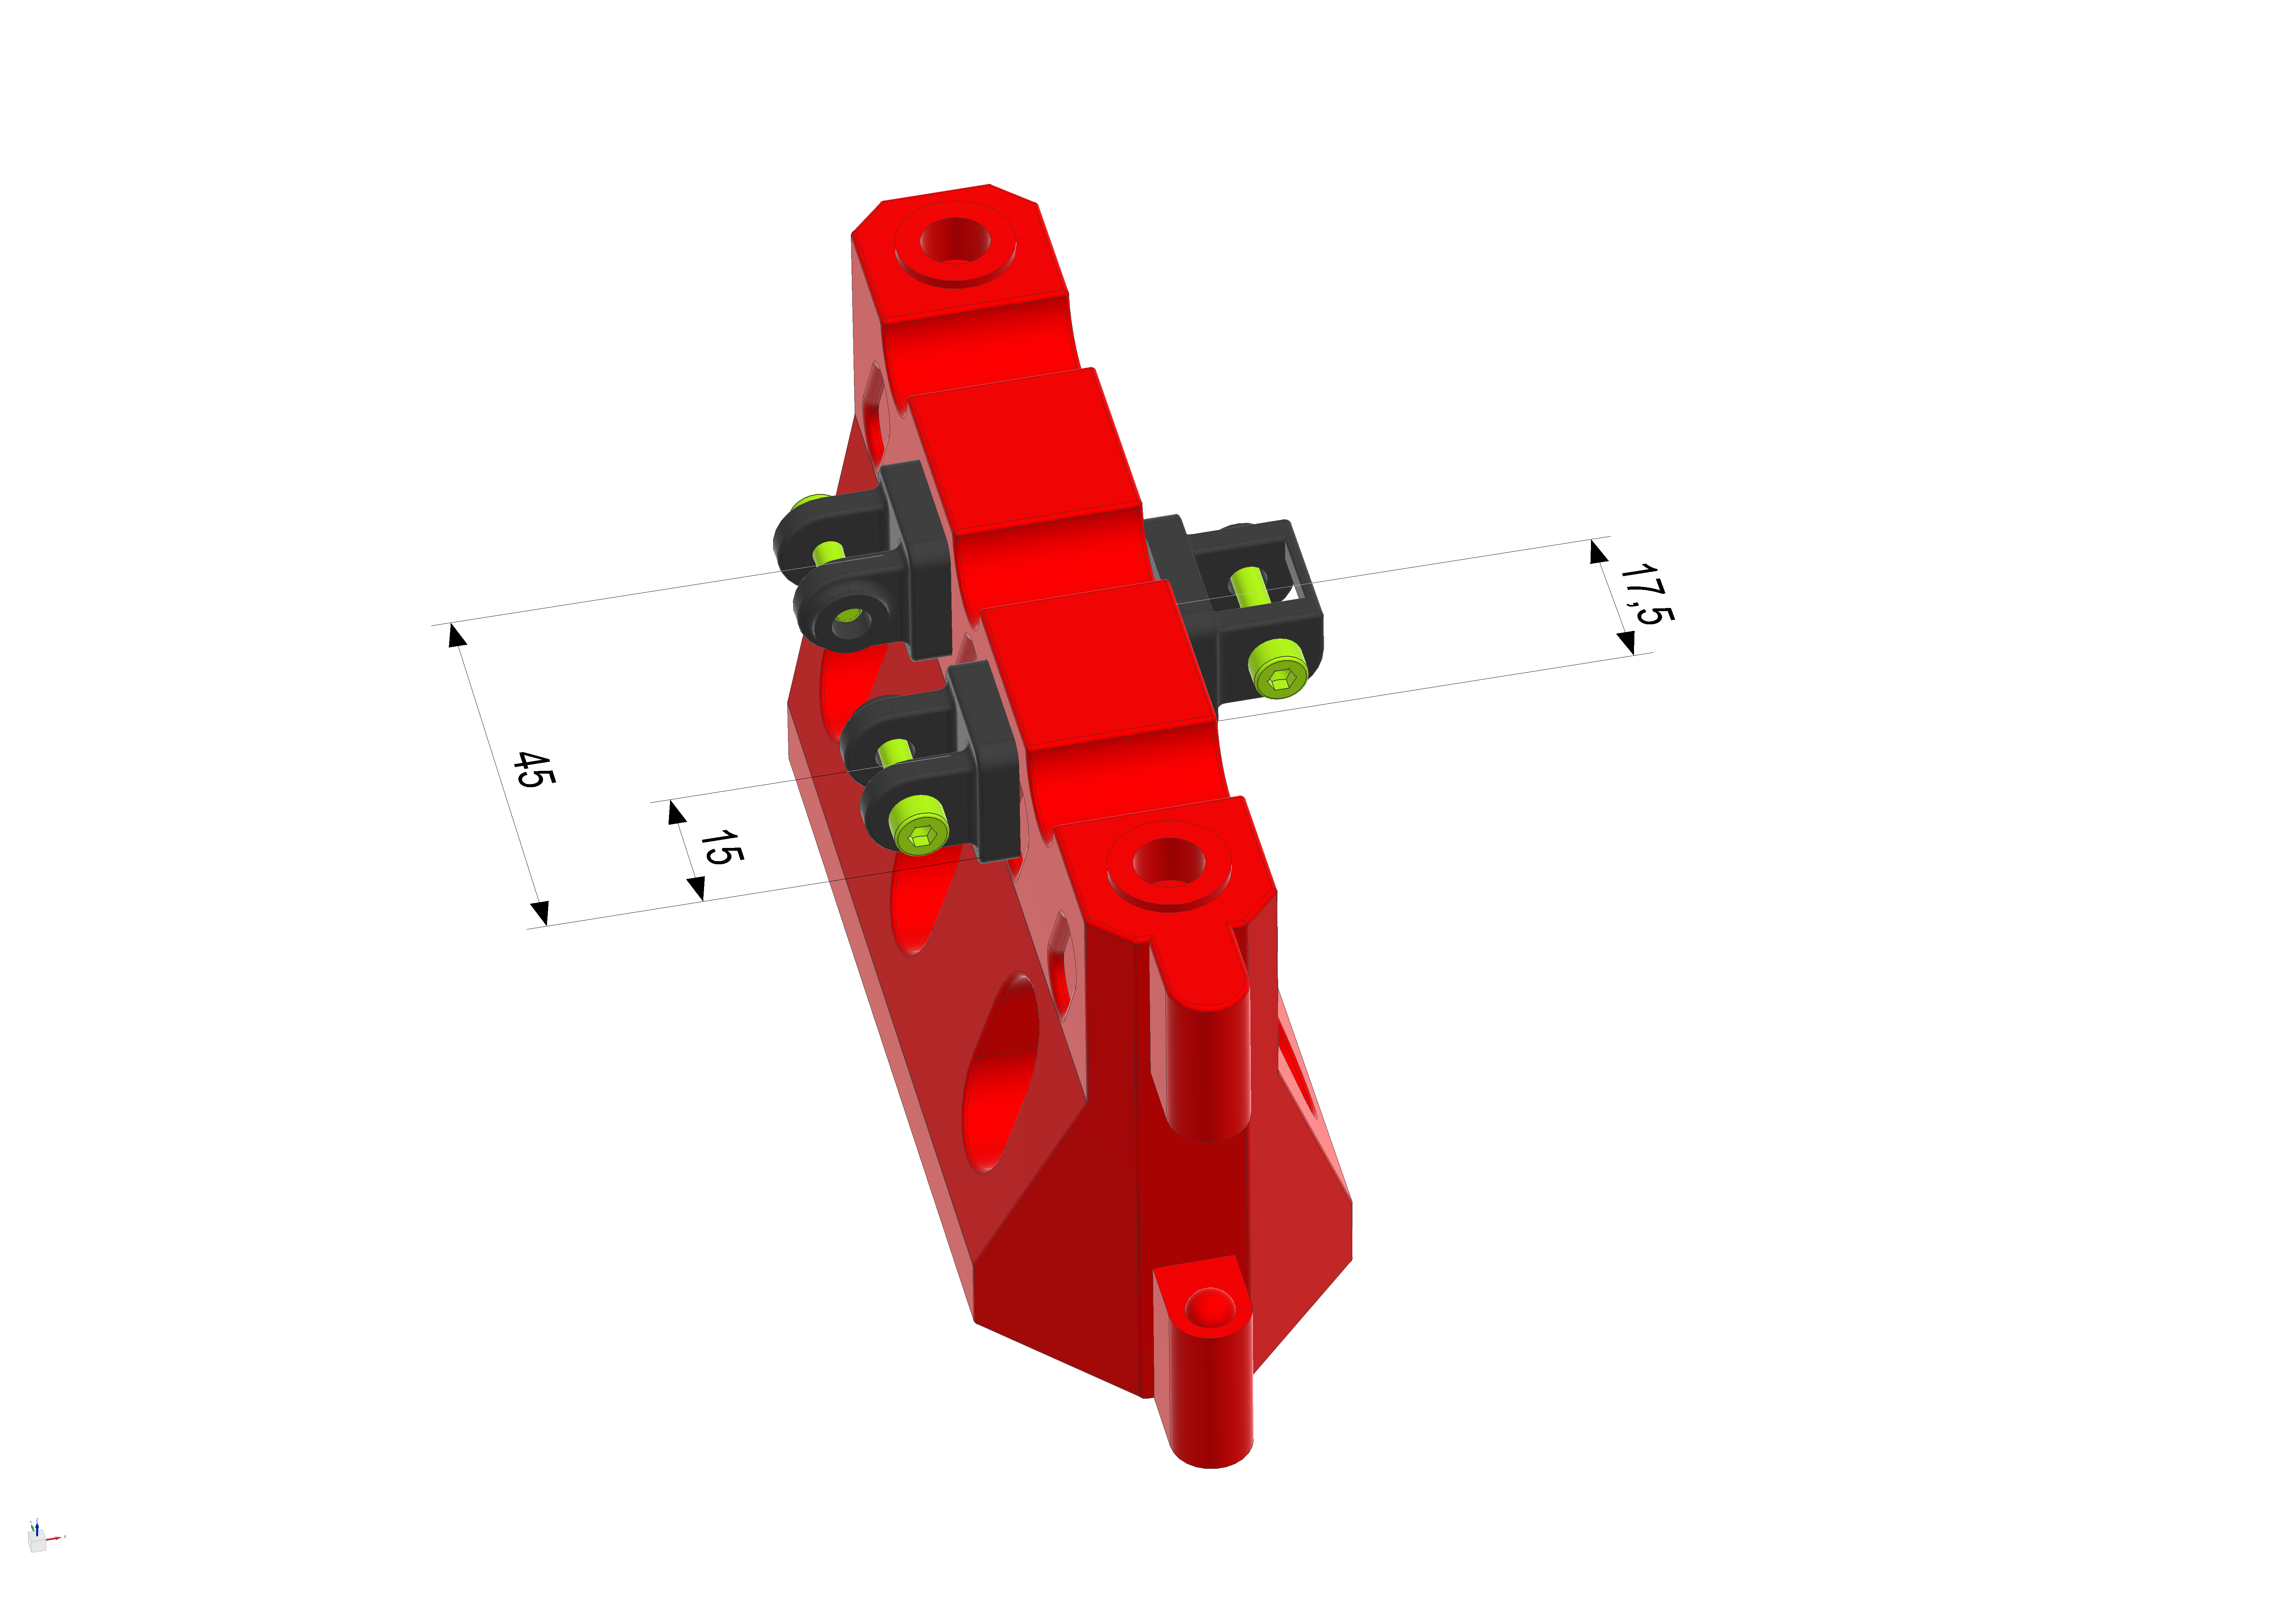
\includegraphics[width=0.95\linewidth]{assets/greifer-prototyp/Greifer_Backen_Trimetric.png} 
\caption{Position Klemmbacken}
\label{fig:obstacle_clamping_concept}
\end{figure}

\newpage

Um sowohl das Klemmen als auch das Anheben des Hindernisses mit einem einzelnen Servomotor zu realisieren, wurde der Mechanismus als ein Gestänge realisiert (Abb. \ref{fig:gripper_components}).

\begin{figure}[H]
\centering
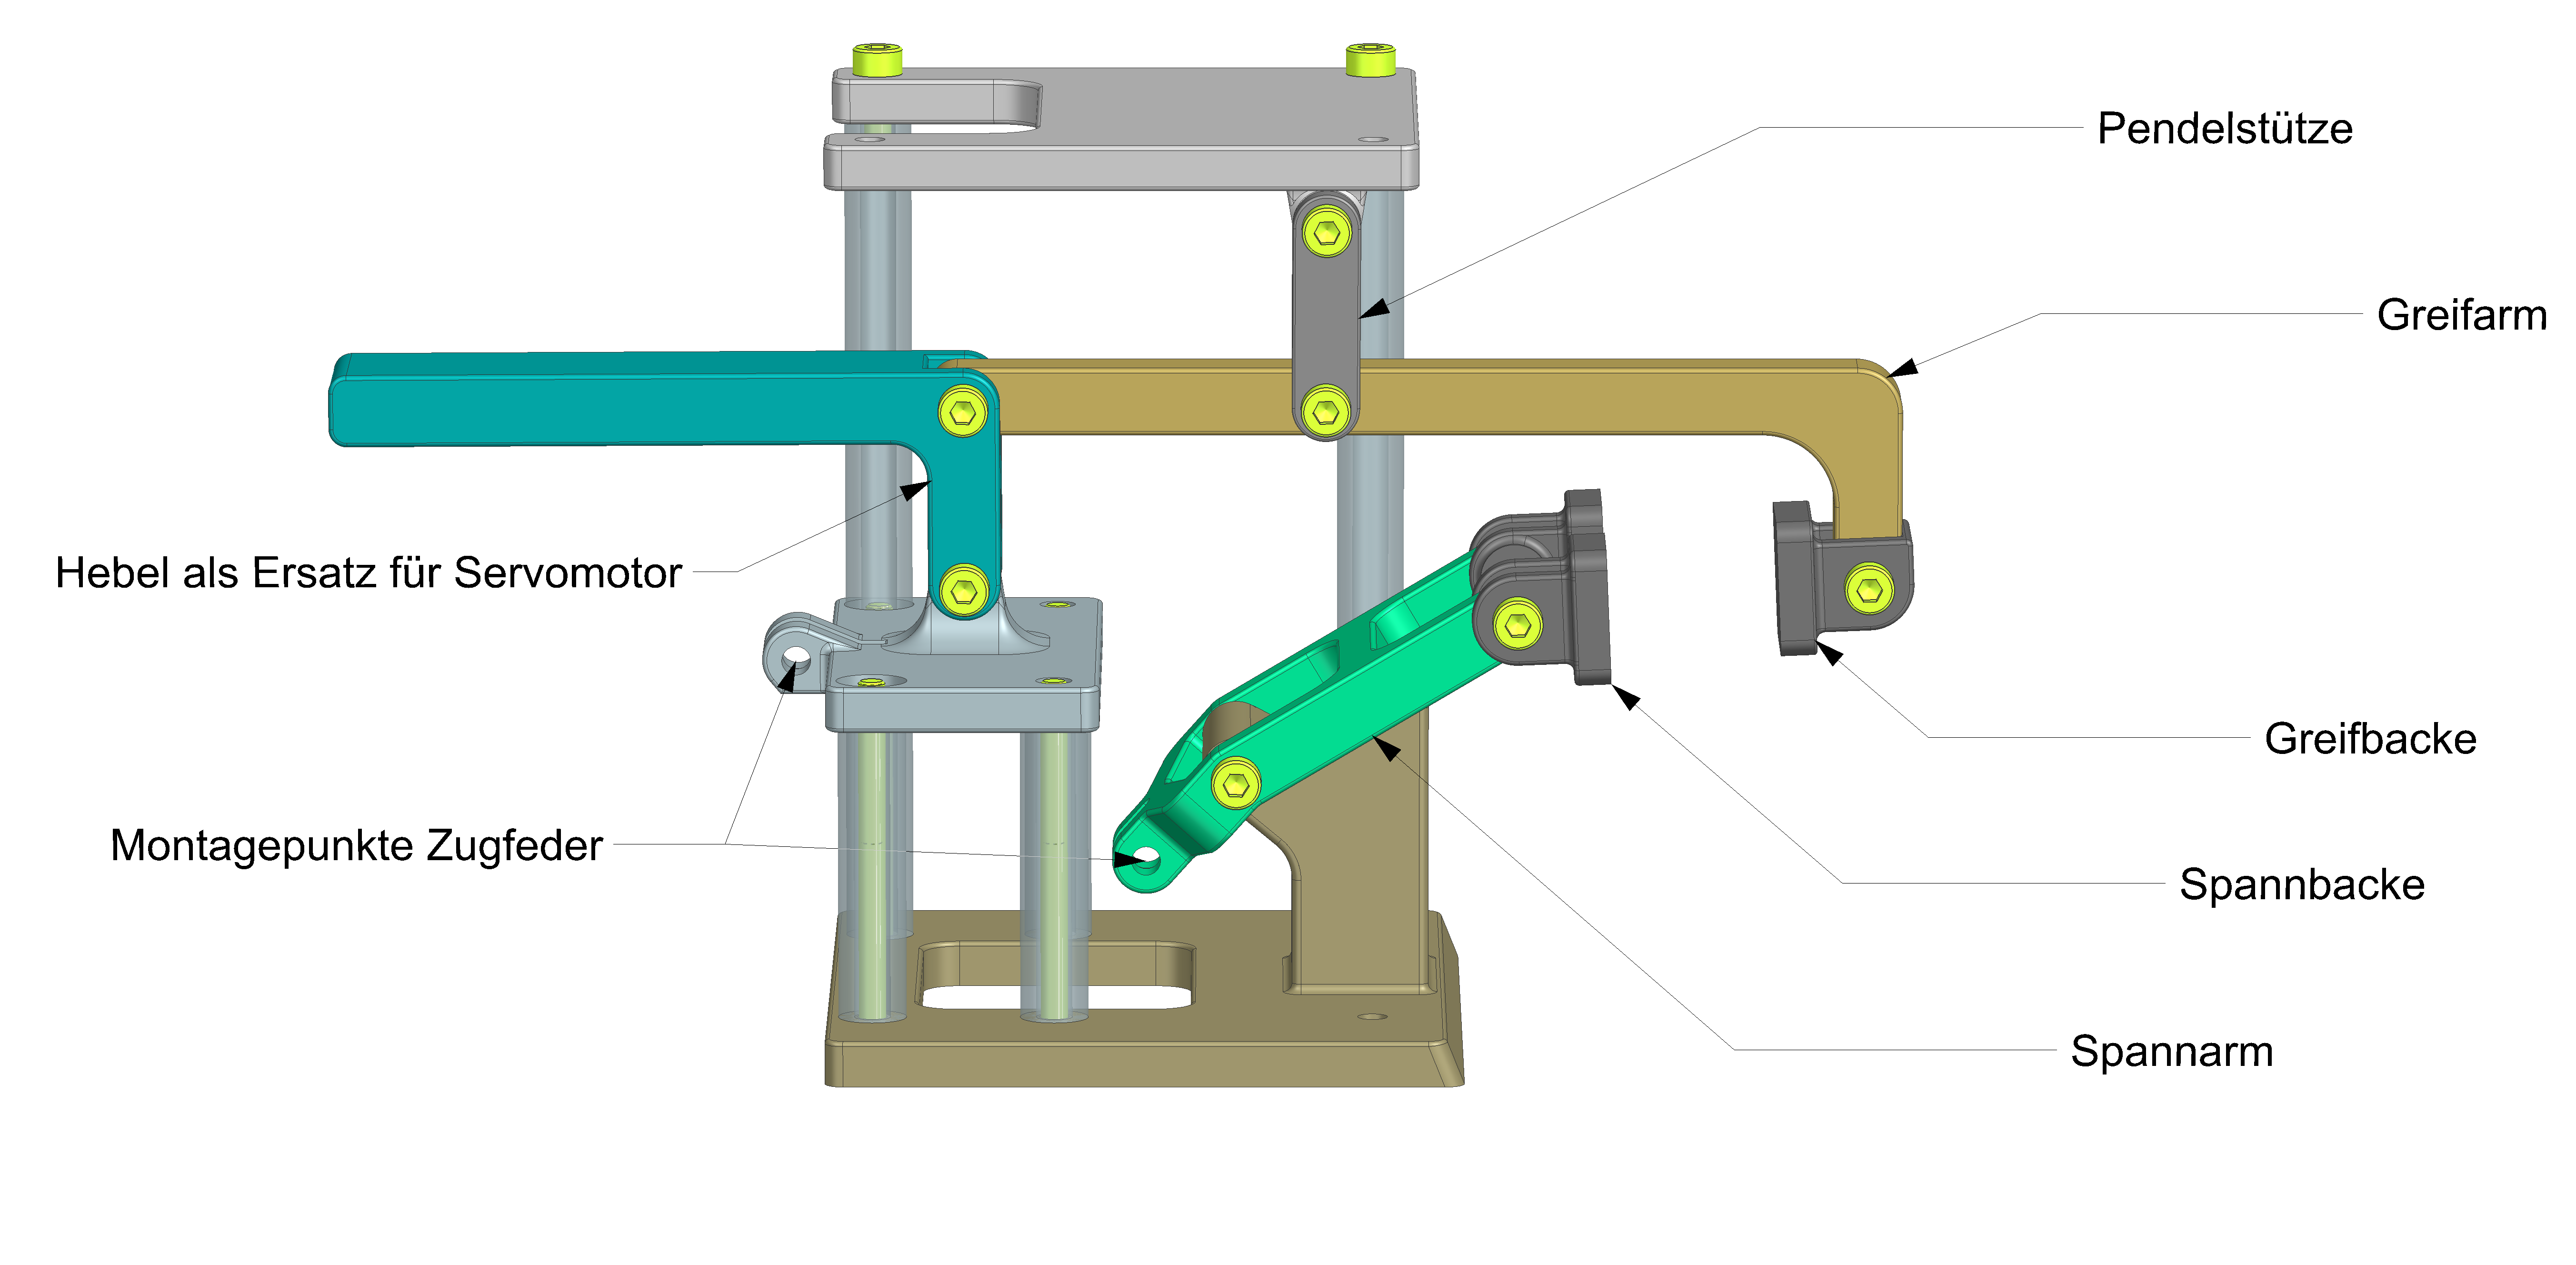
\includegraphics[width=1.0\linewidth]{assets/greifer-prototyp/Greifer_side_Komponentennamen.png} 
\caption{Komponenten des Greifers}
\label{fig:gripper_components}
\end{figure}

Die Greifbacke ist gelenkig mit dem Greifarm verbunden, welcher von der Pendelstütze geführt wird. Am Ende des Greifarms wird der Arm des Servomotors befestigt. Der Servomotor ist in der Abbildung durch einen Hebel ersetzt, da der Prototyp anfangs von Hand bedient wird. Die zwei Spannbacken sind am Spannarm befestigt, welcher drehbar am Chassis des Fahrzeugs gelagert ist und durch eine Zugfeder vorgespannt wird. Abgebildet sind nur die Montagepunkte der Feder.

\newpage

Dreht der Servomotor im Uhrzeigersinn, so schwingen Greifarm und Greifbacke nach oben weg. Der Greifer ist geöffnet (Abb. \ref{fig:gripper_opening_side}). So kann der Roboter auf das Hindernis zu fahren, bis dieses die zwei Spannbacken berührt. An den Spannbacken wird je ein Endschalter montiert, welcher erkennt, wann das Hindernis nahe genug ist und anschliessend den Hebeprozess startet. Dieser Endschlater ist auf der Abbildung \ref{fig:gripper_opening_side} nicht ersichtlich.

Dreht der der Servomotor aus dieser Position im Gegenuhrzeigersinn, so schwingt die Greifbacke zurück, bis sie in Berührung mit dem Hindernis kommt. Dadurch wird das Hindernis gegen die zwei Spannbacken gedrückt, welche wiederum durch die Vorspannung der Feder gegen das Hindernis drücken. Das Hindernis wird eingeklemmt (Abb. \ref{fig:gripper_gripping_side}).

Dreht der Servomotor weiter im Gegenuhrzeigersinn, so dreht nun auch der Spannarm im Gegenuhrzeigersinn mit, da er über das Hindernis vom Greifarm bewegt wird. Die Rotation des Spannarms führt dazu, dass das Hinderniss angehoben wird (Abb. \ref{fig:gripper_lifting_side}). Gleichzeitig wird durch die Rotation des Spannarms die Zugfeder leicht verlängert. Somit wird die Klemmkraft auf das Hindernis erhöht und sichergestellt, dass dieses nicht aus dem Greifer rutscht.

\begin{figure}[H]
\begin{subfigure}{0.55\textwidth}
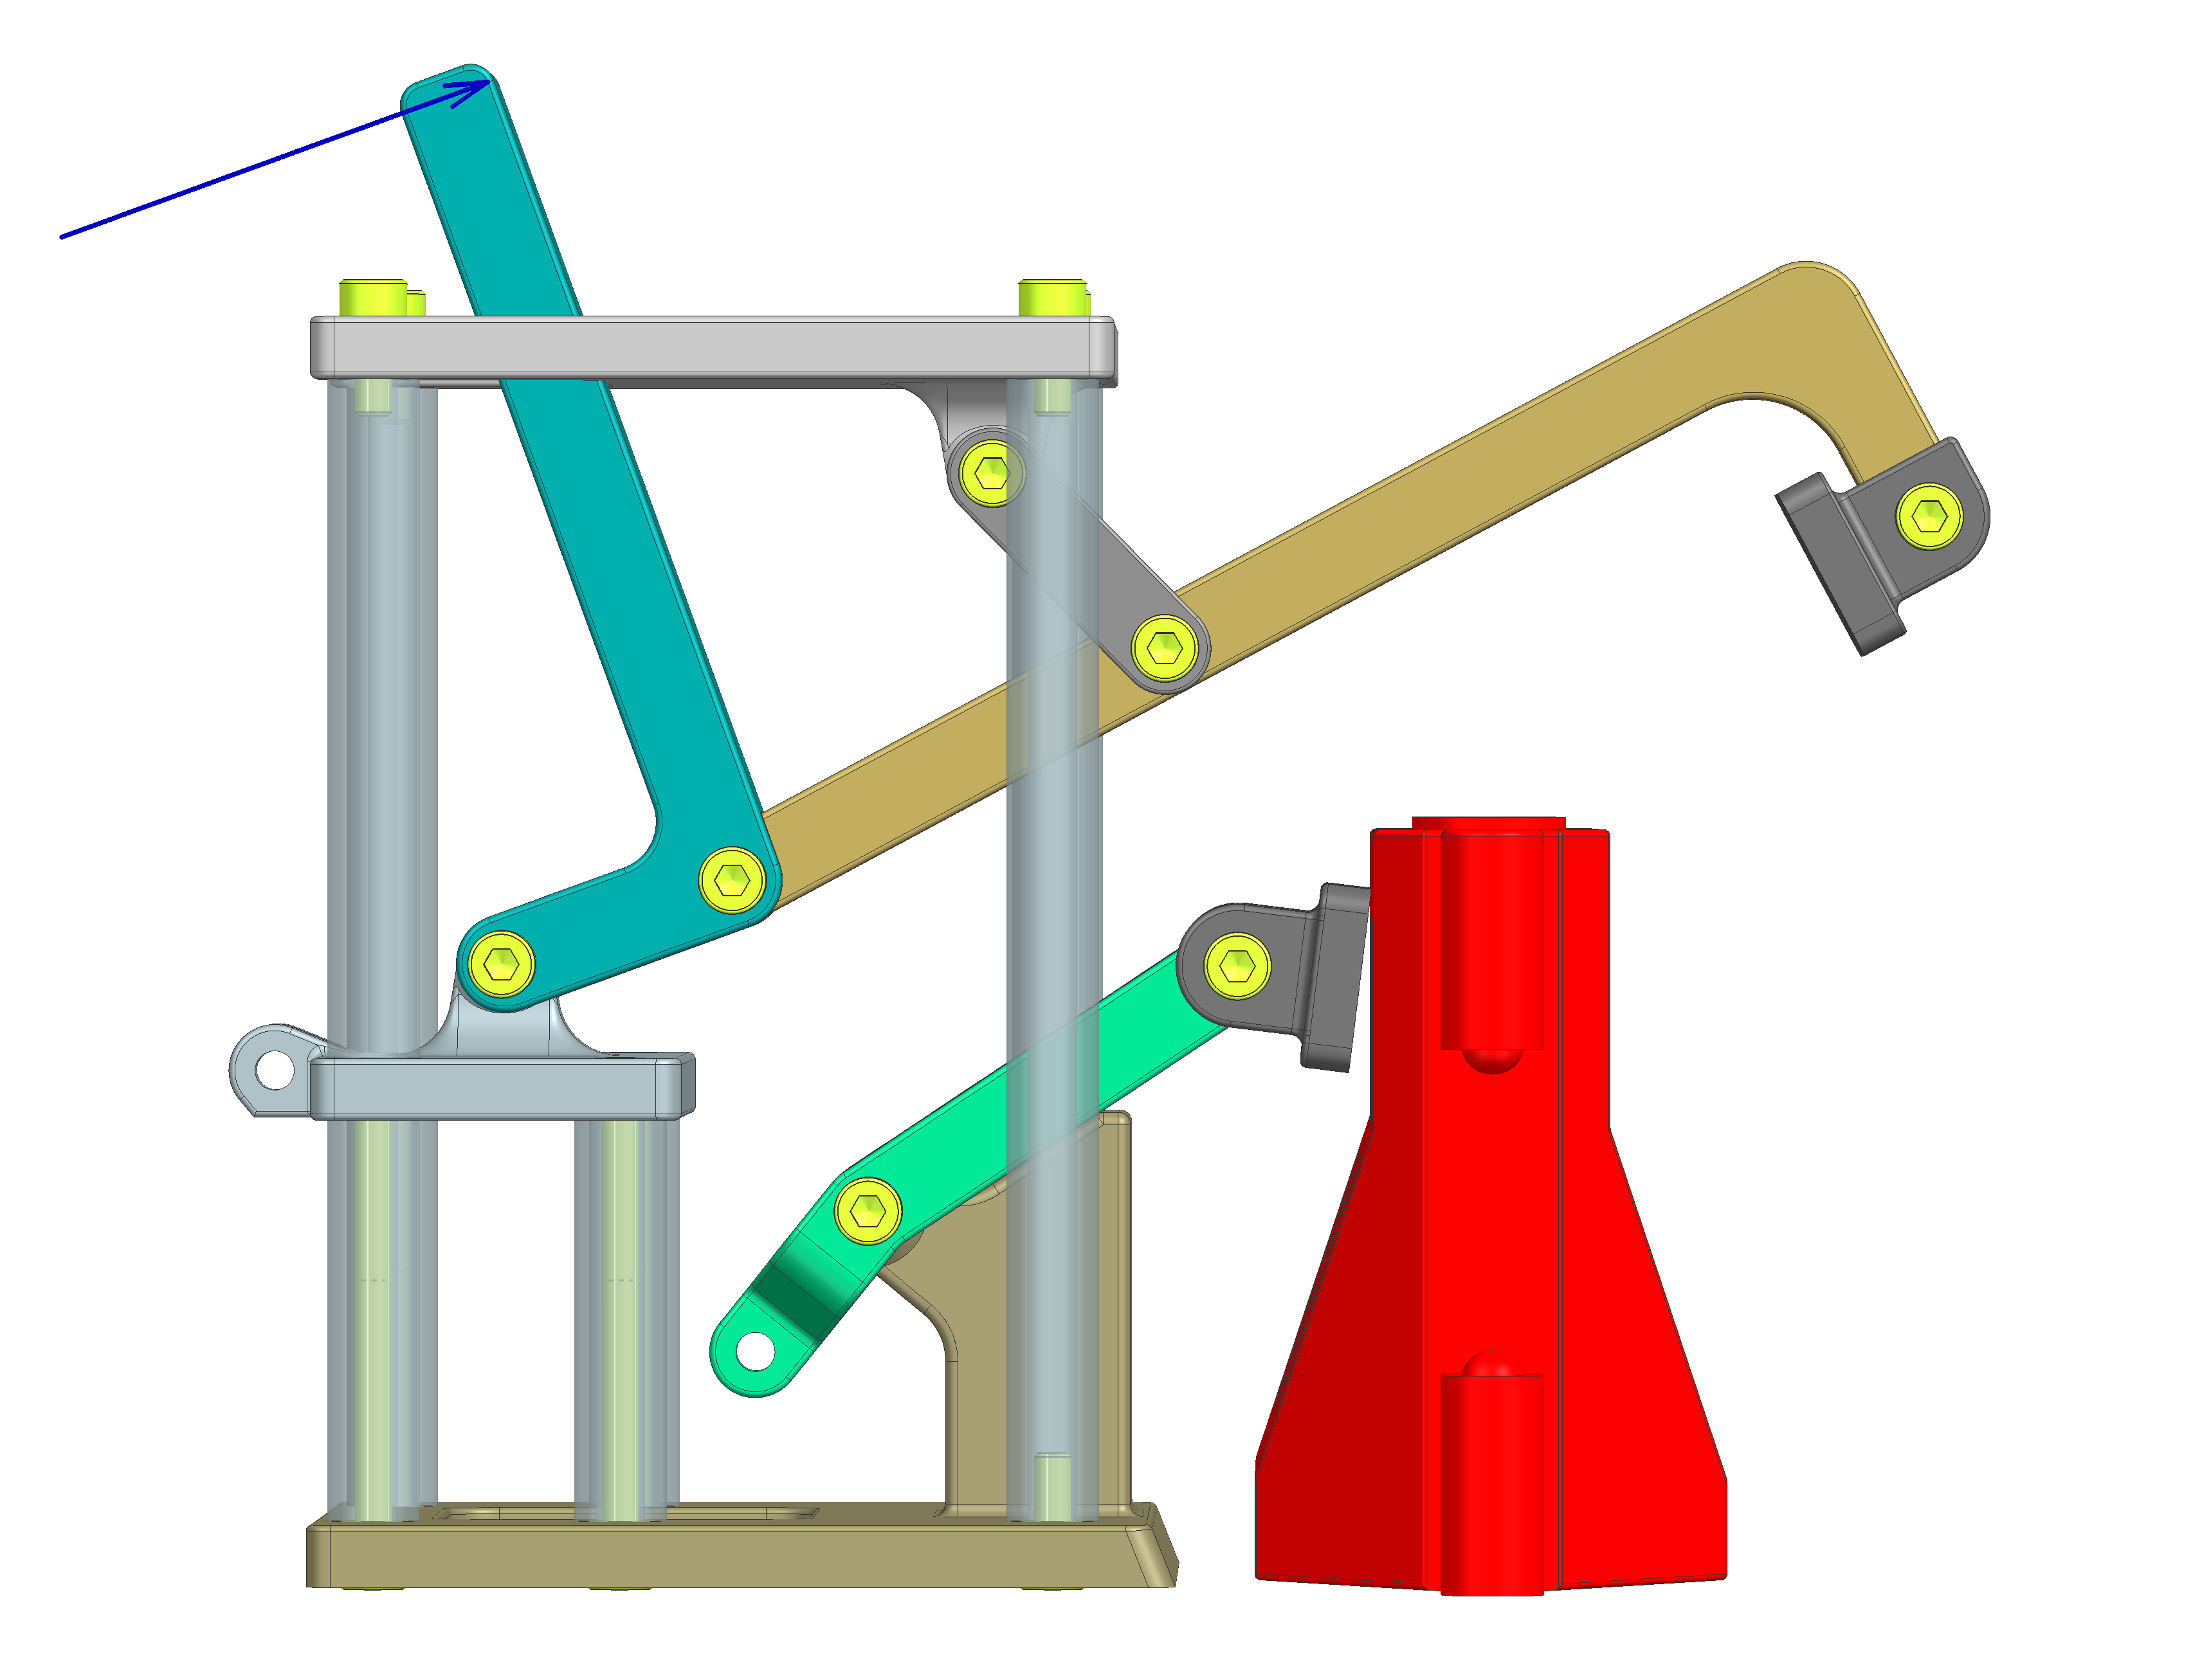
\includegraphics[width=\textwidth]{assets/greifer-prototyp/Greifer_side_Offen.png}
\caption{öffnen}
\label{fig:gripper_opening_side}
\end{subfigure}
\begin{subfigure}{0.55\textwidth}
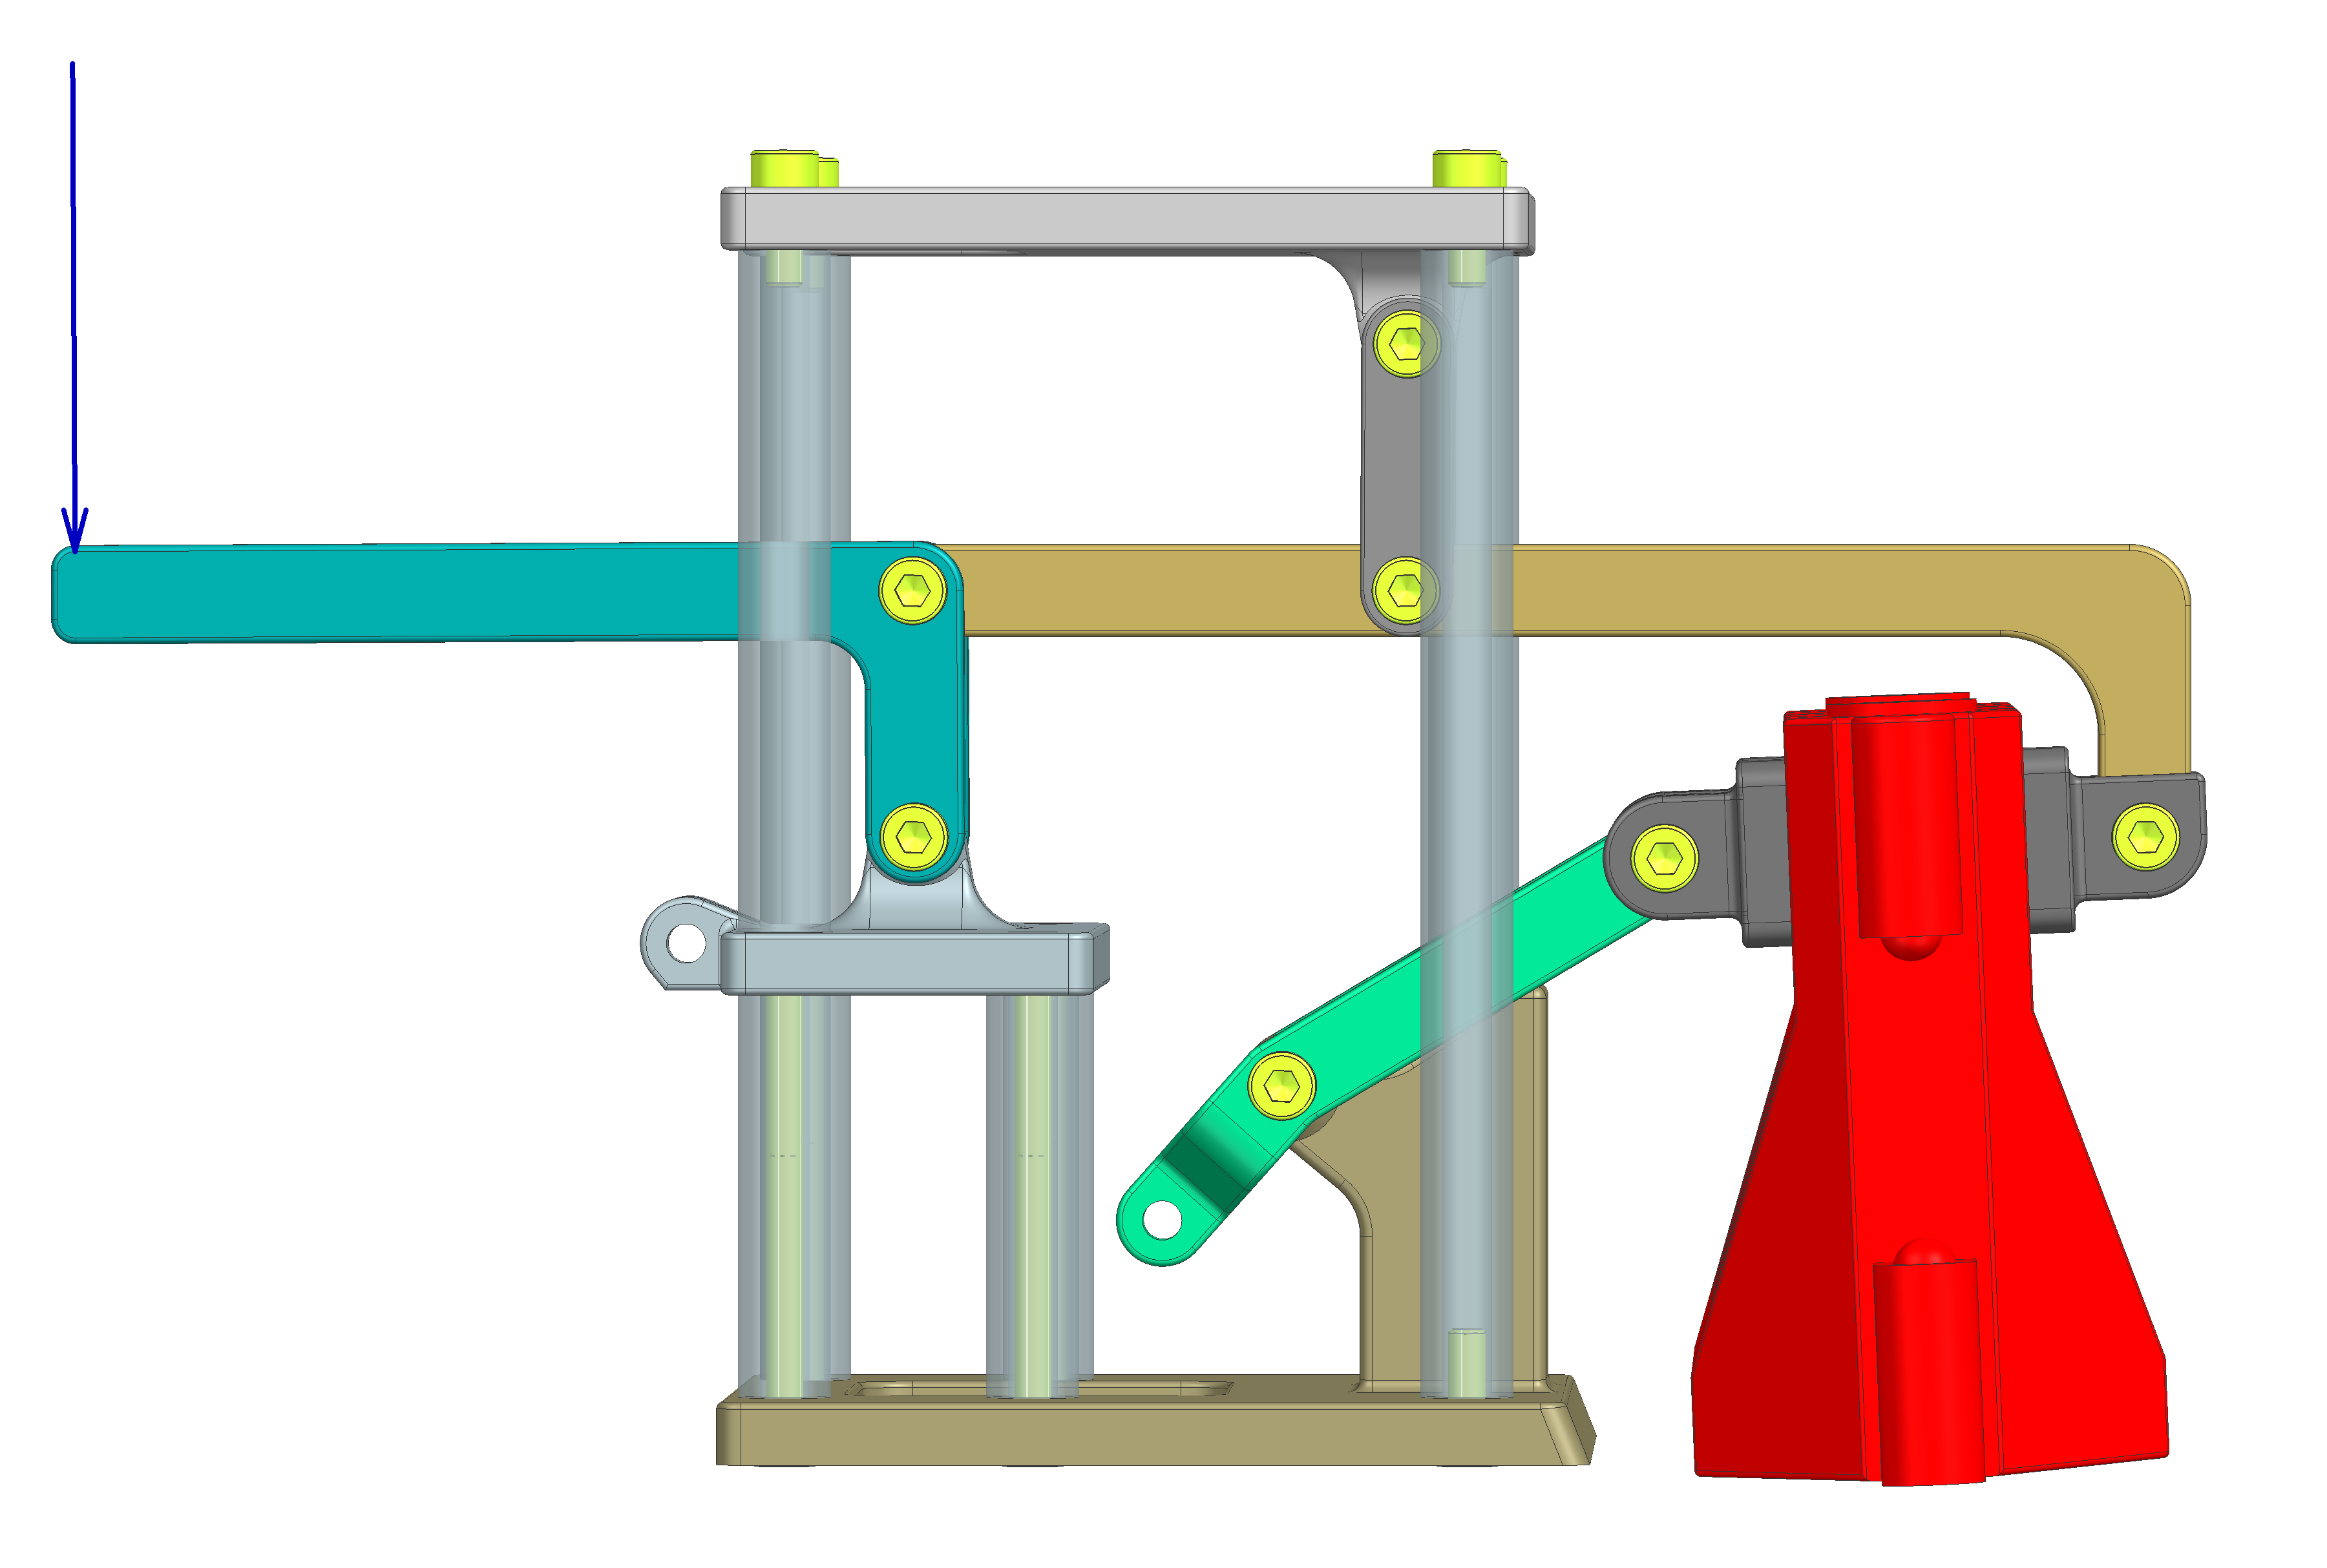
\includegraphics[width=\textwidth]{assets/greifer-prototyp/Greifer_side_Klemmen.png}
\caption{klemmen}
\label{fig:gripper_gripping_side}
\end{subfigure}
\begin{subfigure}{0.55\textwidth}
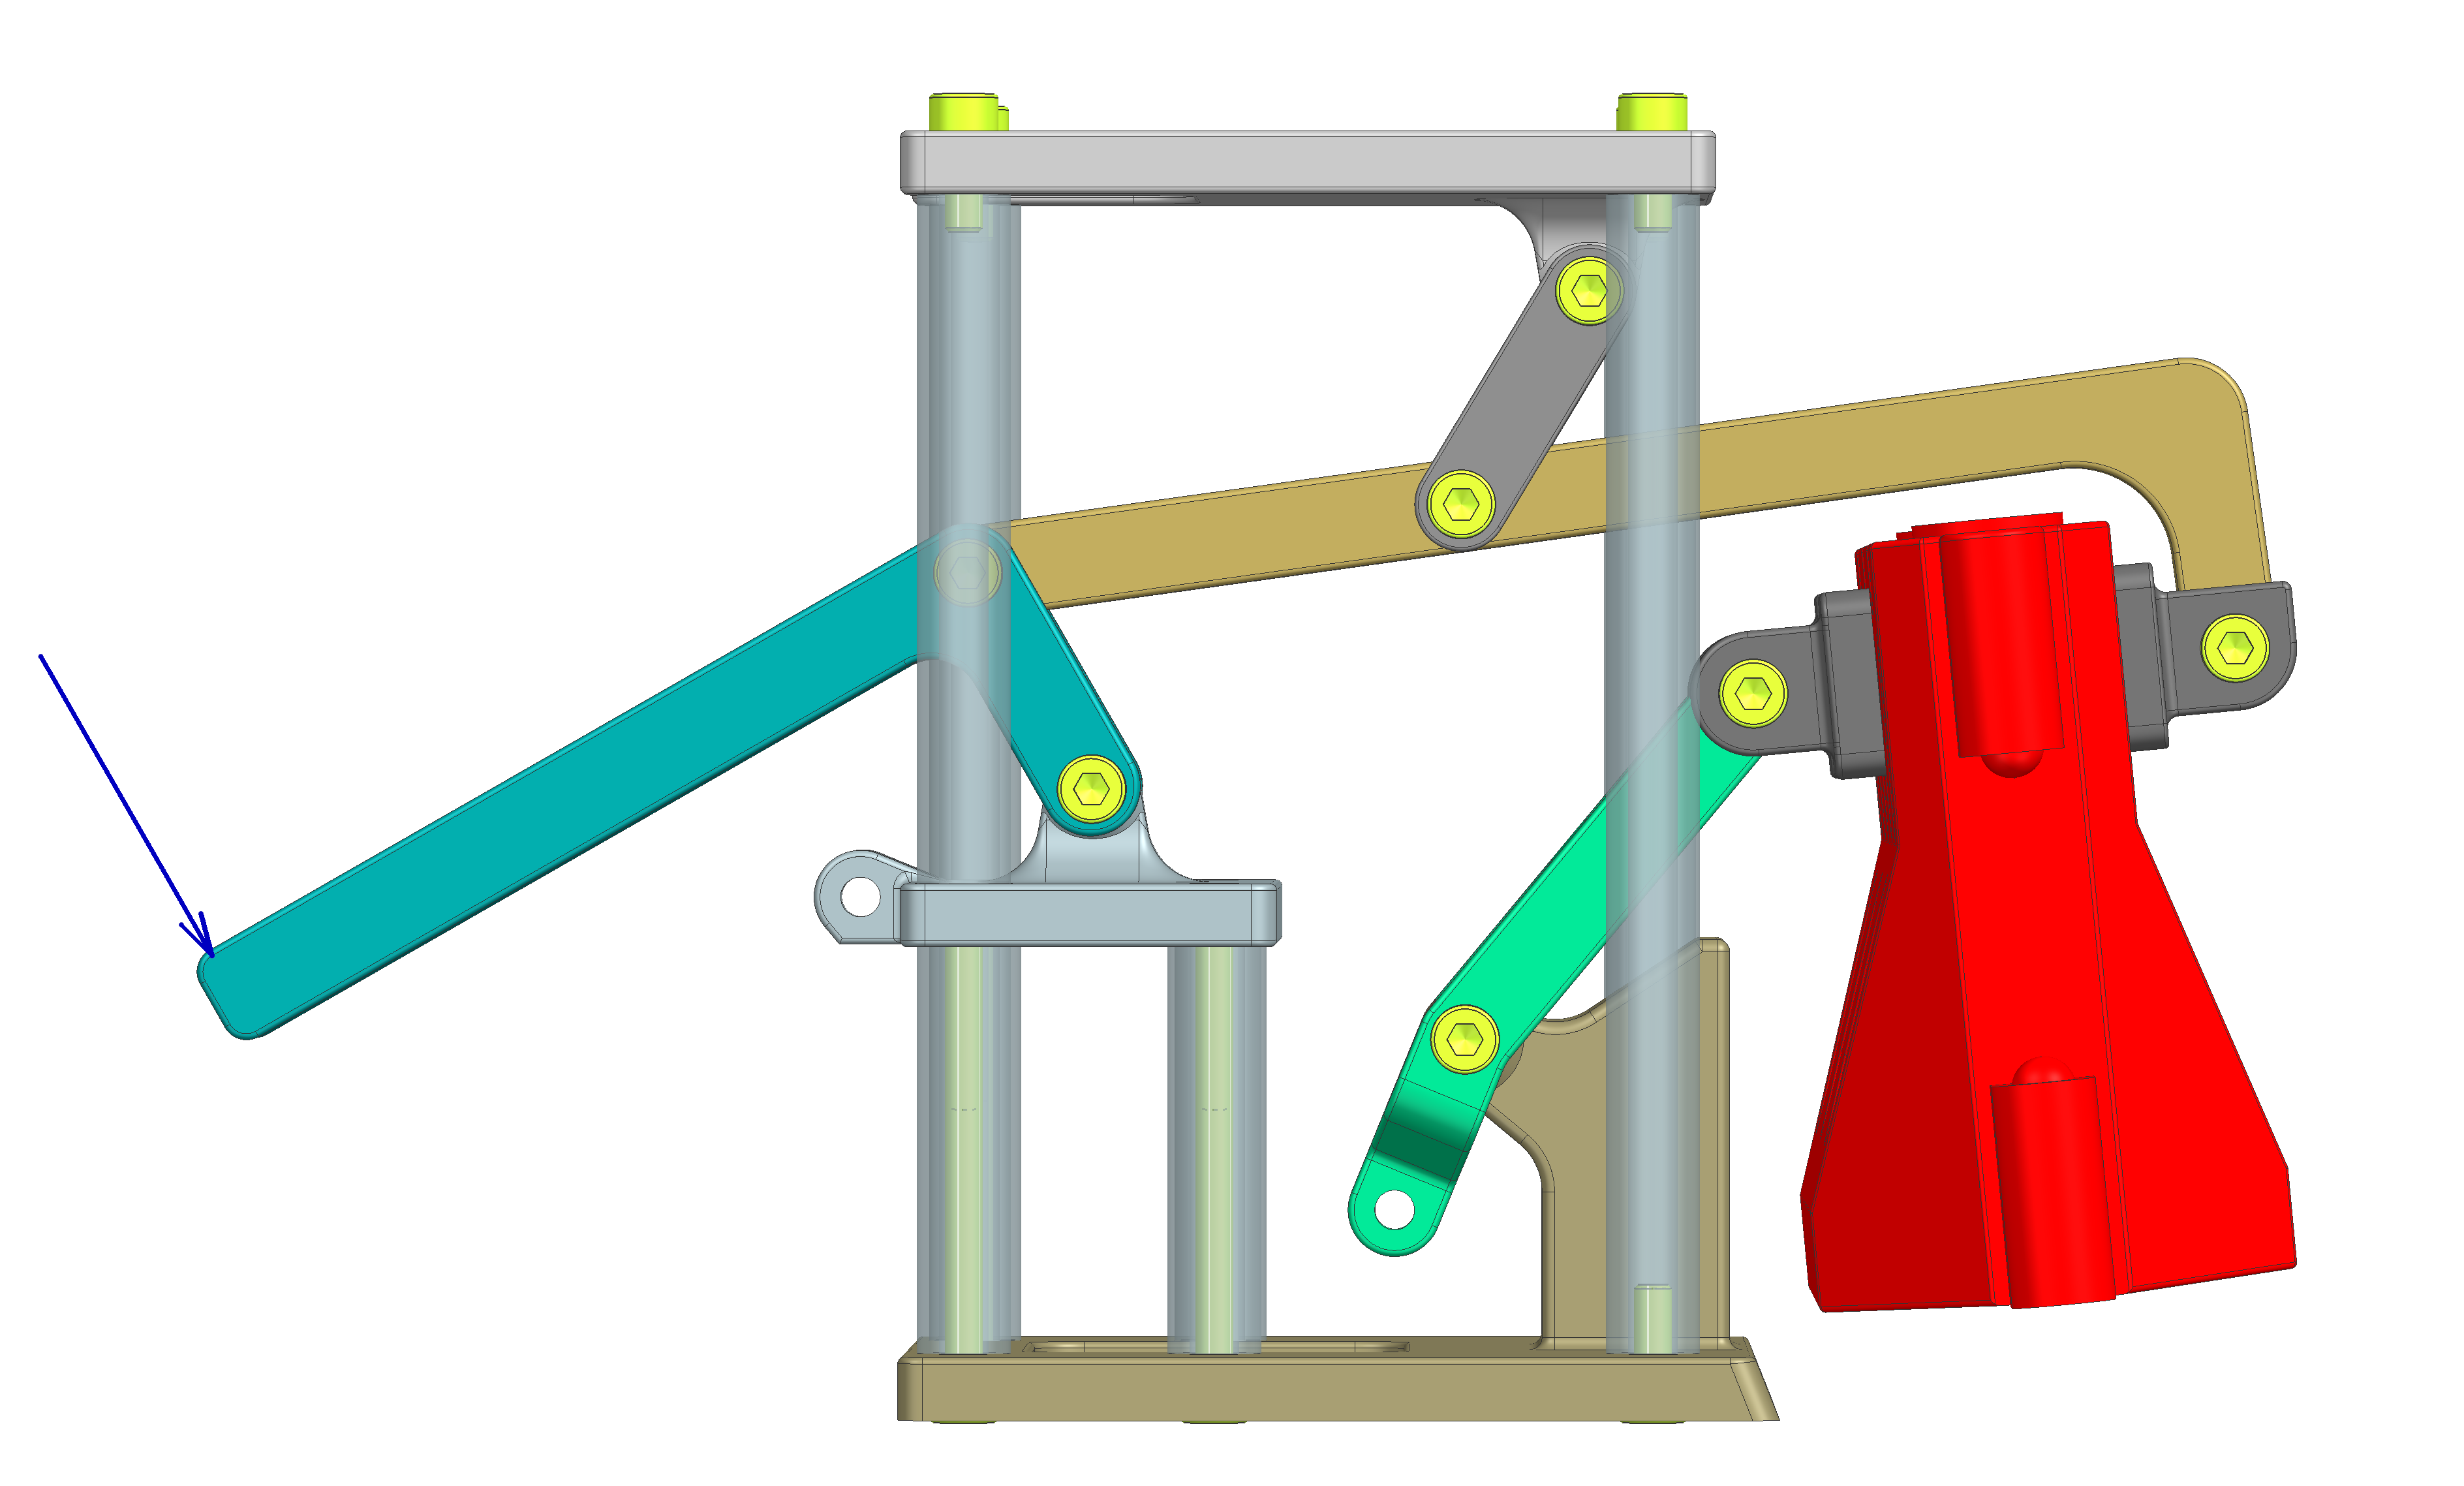
\includegraphics[width=\textwidth]{assets/greifer-prototyp/Greifer_side_Angehoben.png}
\caption{aneheben}
\label{fig:gripper_lifting_side}
\end{subfigure}
\caption{Ablauf Hindernis anheben}
\label{fig:obstacle_gripping_process}
\end{figure}

 \newpage
 
Als Basis zur Auslegung des Greifers dient eine Berechnung der nötigen Klemmkraft, um das Hindernis anzuheben. Dazu wurden ein Haftreibwert von 0.3 zwischen Hindernis und Klemmbacken und eine Sicherheit gegen rutschen von 1.5 angenommen. Mit der Klemmkraft konnte anhand der Geometrie des Greifers eine Feder mit ausreichend hoher Federkonstante ausgewählt werden. Schliesslich wurde zur Auswahl des Servomotors das nötige Drehmoment berechnet, um sowohl die Zugfeder zu verlängern, als auch das Hindernis anzuheben. Die detaillierten Berechnungen sind im Kapitel \textbf{(REF AUSLEGUNG GREIFER)} zu finden. Die Ergebnisse aus den Berechnungen wurden im Kapitel \ref{subsubsection:gripper-prototype-1} anhand eines Prototyps validiert.

Das Klemmen und Anheben ist nur ein Teilschritt  zur Beseitigung eines Hindernisses. Nachfolgend wird der gesamte Ablauf erläutert. Ausgangslage bildet der Ultraschallsensor der das Hindernis erkannt hat und den Prozess einleitet. 

\begin{figure}[H]
\centering
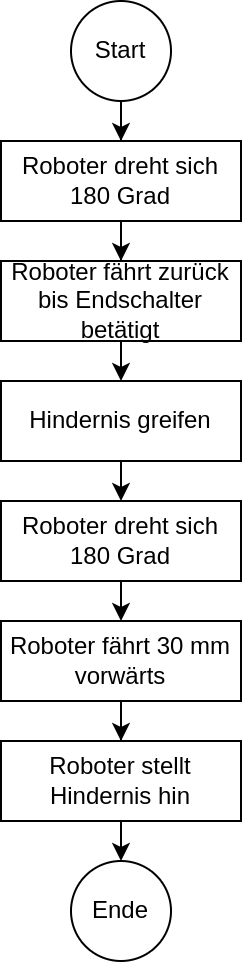
\includegraphics[width=0.2\textwidth]{assets/gesamtkonzept/ablaufdiagramm-hindernis-bewegen.png}
\caption{Ablaufdiagramm Hindernis bewegen}
\label{fig:ablaufdiagramm-hindernis-bewegen}
\end{figure}

 Mit einem Ultraschall-Sensor soll das Vorhandensein eines Hindernisses und die ungefähre Distanz dazu bestimmt werden. Zur genauen Bestimmung der Distanz vor dem Greifer wird der Endschalter am Greifmechanismus verwendet.
Greifer und Endschalter werden sich an der Rückseite des Fahrzeugs befinden, der Ultraschallsensor vorne (siehe Abb. \ref{fig:robot_concept-scetch_labeld}). Dadurch muss sich das Fahrzeug, nachdem ein Hindernis mittels Ultraschall entdeckt wurde, 180\textdegree\ drehen und langsam rückwärts fahren, bis der Endschalter am Greifer betätigt wird, um das Hindernis anzuheben. Sobald das Hindernis angehoben ist, dreht sich das Fahrzeug 180\textdegree\ und fährt 30mm vorwärts, um das Hindernis an dieselbe Stelle zurück zu setzen. Das Fahrzeug steht nach dem Absetzen wieder nach vorne ausgerichtet und kann geradeaus weiter fahren (siehe  Abb. \ref{fig:ablaufdiagramm-hindernis-bewegen}).


\subsection{Fortbewegung}

Das Fahrzeug wird mit zwei einzeln angesteuerten Räder angetrieben. Die DC-Motoren besitzen Encoder und sind direkt mit den Antriebsrädern verbunden.  Dadurch kann genau festgestellt werden welche Distanz zurückgelegt wurde. Der Fahrbefehl entsteht aufgrund der Berechnungen der Bilderkennung. Dem Mikrocontroller \acrshort{tinyk22}, der die Motoren ansteuert,  werden Distanz und Drehwinkel mitgeteilt.

\subsection{Linienerkennung}

Mit einem Array von Phototransistoren,  Kondensatoren und Widerständen misst man die Entladezeit mittels Mikrocontroller und der Input Capture Funktion. Der Liniensensor dient als Unterstützung damit man die Linie nicht verlässt während dem Fahren. Jedoch ist das Ziel den Robotor gerade vor der Linie zu positionieren, so dass der Liniensensor theoretisch nicht gebraucht wird während des Fahrens. Ein weiterer Nutzen benötigt man um zu prüfen ob man auf einem Knoten steht oder nicht.

\subsection{Distanzsensor}

Um die Distanz zwischen dem Roboter und einem Hindernis zu detektieren wird ein Ultraschallsensor verwendet. Somit kann man erkennen an welchem Punkt das Fahrzeug eine 180-Grad-Drehung durchführen muss, um sich auf den Hubvorgang vorzubereiten. Ebenfalls wird so ein Zusammenstossen mit Hindernissen verhindert, falls diese bei der Bilderkennung zuvor nicht erkannt wurde.

\subsection{Wegfindung}

Der kürzeste Weg im Graphen vom momentanen Knoten zum Zielknoten wird mit dem Dijkstra Algorithmus\footnote{\url{https://www.w3schools.com/dsa/dsa\_algo\_graphs\_dijkstra.php}} berechnet. Dieser wird zu Beginn berechnet und jedes Mal, wenn der Roboter neue Erkenntnisse zum Graph gesammelt hat, aktualisiert. 

Zusätzlich zum zukünftigen Pfad, wird der bereits befahrene Pfad gespeichert. Dies dient dazu, dass der Roboter immer in der Lage sein wird, im Fehlerzustand, auf den letzten Knoten zurückzufahren und dabei die Orientierung beibehält.

\subsection{Kameraposition}

Die Kamera wird in einer Höhe von ca. 22.5cm und einem Winkel von ca. 56\textdegree\ montiert. Die Position ist fix, das heisst, wir benötigen keine schwenkbare Kamera. In der folgenden Grafik \ref{fig:camera-position-concept} ist die Kameraposition ersichtlich. Die Kamera selbst verfügt über ein Horizontales Field of View\footnote{\url{https://en.wikipedia.org/wiki/Field_of_view}} von 66\textdegree. Wir verwenden die Kamera im Hochformat, Somit haben wir im Field of View von 66\textdegree\ sowohl sehr nahe Knoten und Objekte bis zu 10cm im Bild. Aber auch weit entfernte Pylonen, welche 200cm entfernt stehen.

\begin{figure}[H]
    \centering
    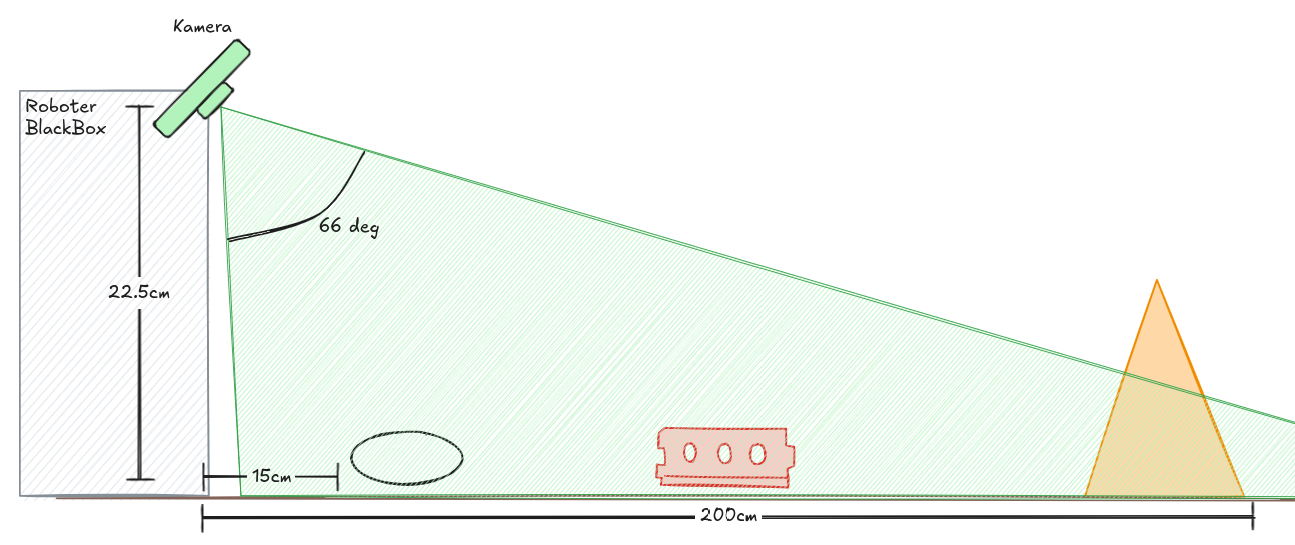
\includegraphics[width=1\linewidth]{assets//informatik-prototyp//camera/camera_position.png}
    \caption{Kamera Positionierung}
    \label{fig:camera-position-concept}
\end{figure}



\newpage

\subsection{Schnittstellen zwischen den Kompontenten}

Im Blockschaltdiagramm in Abbildung \ref{Blockdiagramm Steuerung} wird die Hardware der Steuerung aufgezeigt. Die genauen Funktionen des Mikrocontroller sind im Prototyping Kapitel \ref{Blockdiagramm: Schnittstellen zwischen den Komponenten} beschrieben. Im Zentrum steht der Mikrocontroller \acrshort{tinyk22}.  Er steuert und verarbeitet die Signale der verschiedenen Komponenenten wie Motoren, Ultraschallsensor, Liniensensor oder Motortreiber. Die Verbindung zum Raspbberry Pi, der die Bilder auswertet,  wird über \acrfull{uart} aufgebaut. Die Stromüberwachung sorgt dafür, dass keine elektrischen Komponenten durch Überlast beschädigt werden.




\begin{figure}[H]
    \centering
    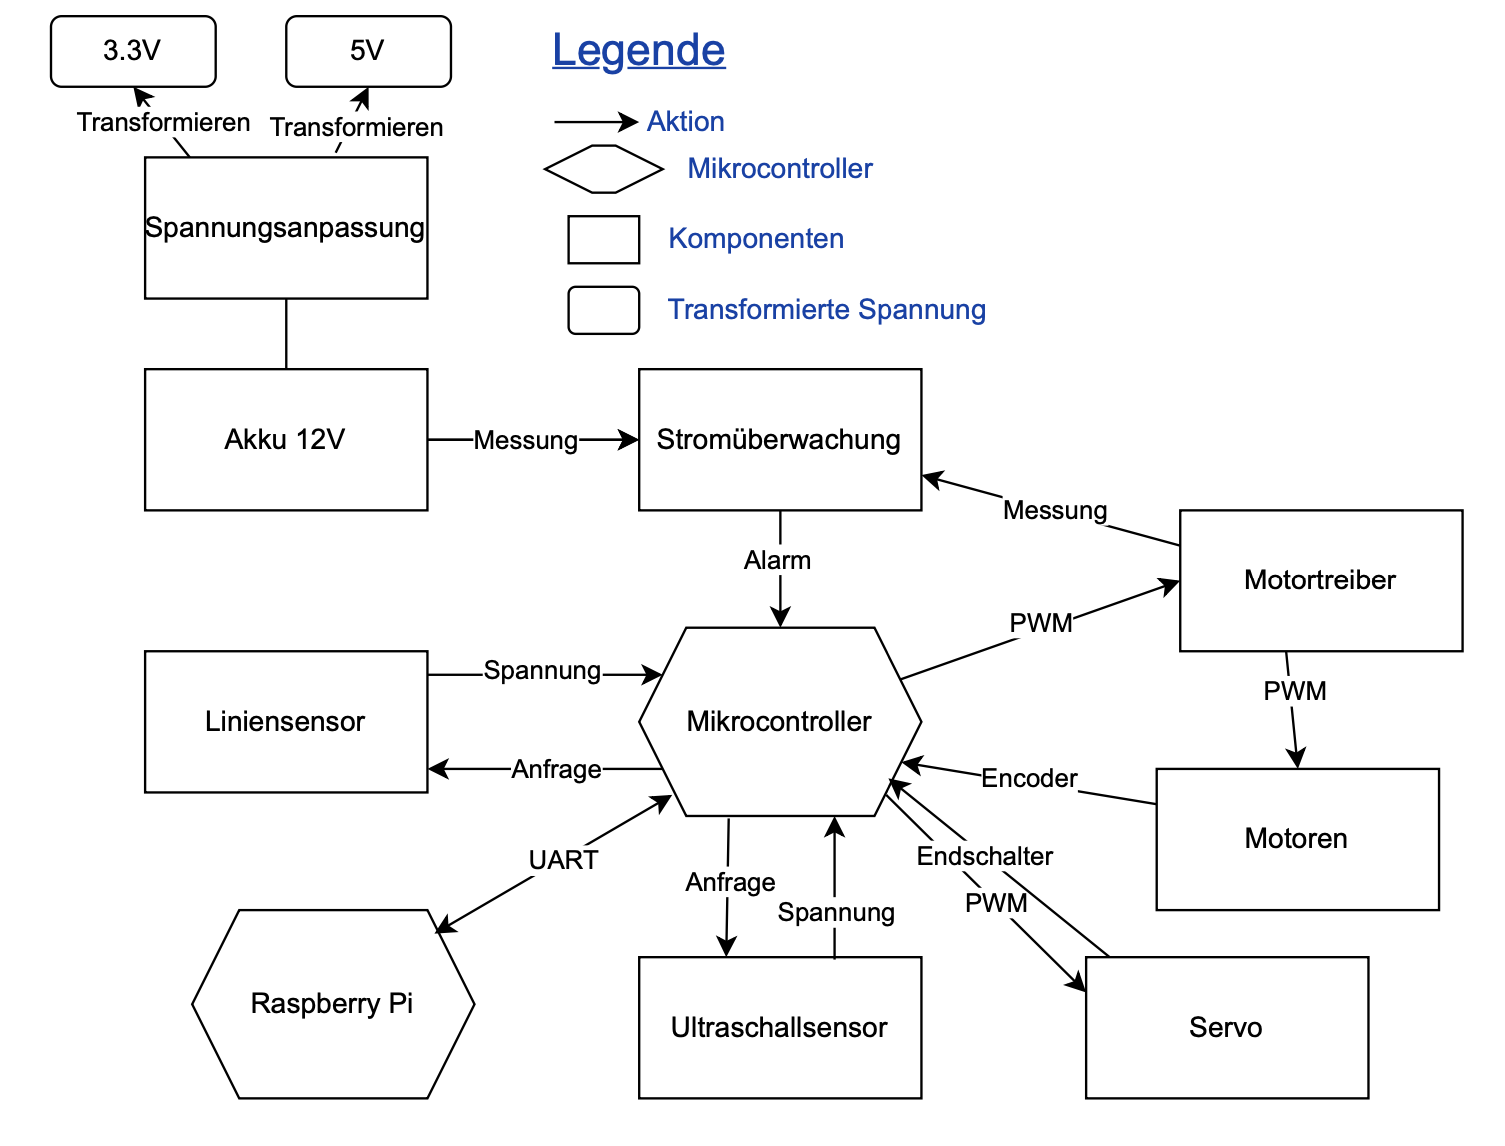
\includegraphics[width=1\linewidth]{img/Blockdiagramm-ET-drawio.drawio-2.png}
    \caption{Blockdiagramm Steuerung}
    \label{Blockdiagramm Steuerung}
\end{figure}


